% Conceptual foundations, restructured 12 October 2026.
\chapter{Foundations}
\label{chap:foundations}
\chaptermark{Foundations}
\begingroup
\clubpenalty=10000
\widowpenalty=10000
% Keep at least three lines of a split paragraph on either side.
\clubpenalties 3 10000 10000 0
\widowpenalties 3 10000 10000 0
\displaywidowpenalty=10000
\postdisplaypenalty=10000
\raggedbottom

Energy management combines physical assets, information about their condition, and decisions whose consequences unfold over time. The thesis investigates \gls{marl} for coordinating these decisions in \glspl{rec}, bringing energy-domain concepts together with the foundations of learning and decision-making.

The chapter first establishes the energy-domain concepts and the neural networks used to represent learned functions. It then introduces single-agent \gls{rl} and \gls{marl} before considering recorded experience, hierarchical decisions, and structured policy architectures. These foundations prepare the reader for the analysis of existing methods in Chapter~\ref{chap:related-work} and for the controller formulations developed later in the thesis.

\FloatBarrier
\section{Renewable Energy Communities}
\label{sec:ch2-rec}

This section introduces the energy-domain concepts used throughout the thesis to help the reader follow the later discussion. It begins with \gls{rec} members and their organisation, then examines asset operation, flexibility, and market signals before describing the information and conditions needed for operation.

\Needspace{7\baselineskip}
\subsection{Community Members}
\label{sec:ch2-rec-members}
\label{sec:ch2-community-structure}

A \emph{\gls{rec} member} is a person or organisation participating in the \gls{rec}'s activities under its membership arrangements. Members can take different energy roles. A \emph{consumer} uses electricity, a \emph{producer} generates it, and a \emph{prosumer} combines both activities. A household with rooftop \gls{pv} panels may therefore be a prosumer while drawing electricity from the grid during the evening. Membership describes participation in the collective; the energy role describes the member's activities \parencite{reis2021businessmodels}.

Those activities take place at a \emph{site}, which is a physical installation, such as a dwelling, commercial building, or industrial facility, with one or more connections to the electricity grid. The individual units of energy equipment within a site are termed \emph{assets}, including chargers, batteries, and \gls{pv} panels. A member may be associated with several sites, while a shared building may accommodate several members. Assets can also be collectively owned or used, as with a \gls{rec} battery or a charging facility serving several households \parencite{moret2019energycollectives,reis2021businessmodels}.

Section~\ref{sec:intro-energy-flexibility} described a household scheduling the charging of an \gls{ev} around its daily activities. In that example, the people living in the house participate as a \gls{rec} member, and their home is the site. The charger is an asset installed at the site, and the \gls{ev} connects to it during a charging session. These terms distinguish the participant, the installation, and the individual assets whose operation is managed there. The broader term \emph{energy resource} refers to the supply, storage capability, or demand available to the control problem. Assets provide these resources, whose availability also depends on operating status and service requirements.

The organisation extends from these individual assets to the wider electricity system. Assets operate within sites, sites participate in \glspl{rec}, and their exchanges with the grid involve the distribution and transmission networks. This hierarchy gives each level a different scope of operation, as illustrated in Figure~\ref{fig:ch2-community-structure}.

Above the \gls{rec} level, network operators manage the infrastructure through which sites exchange electricity. The \gls{dso} operates, maintains, and develops the distribution network serving connected users. The \gls{tso} performs these functions for the transmission network and its interconnections, supporting secure operation across the wider system \parencite{eu2019electricity}.

\begin{figure}[!htbp]
\centering
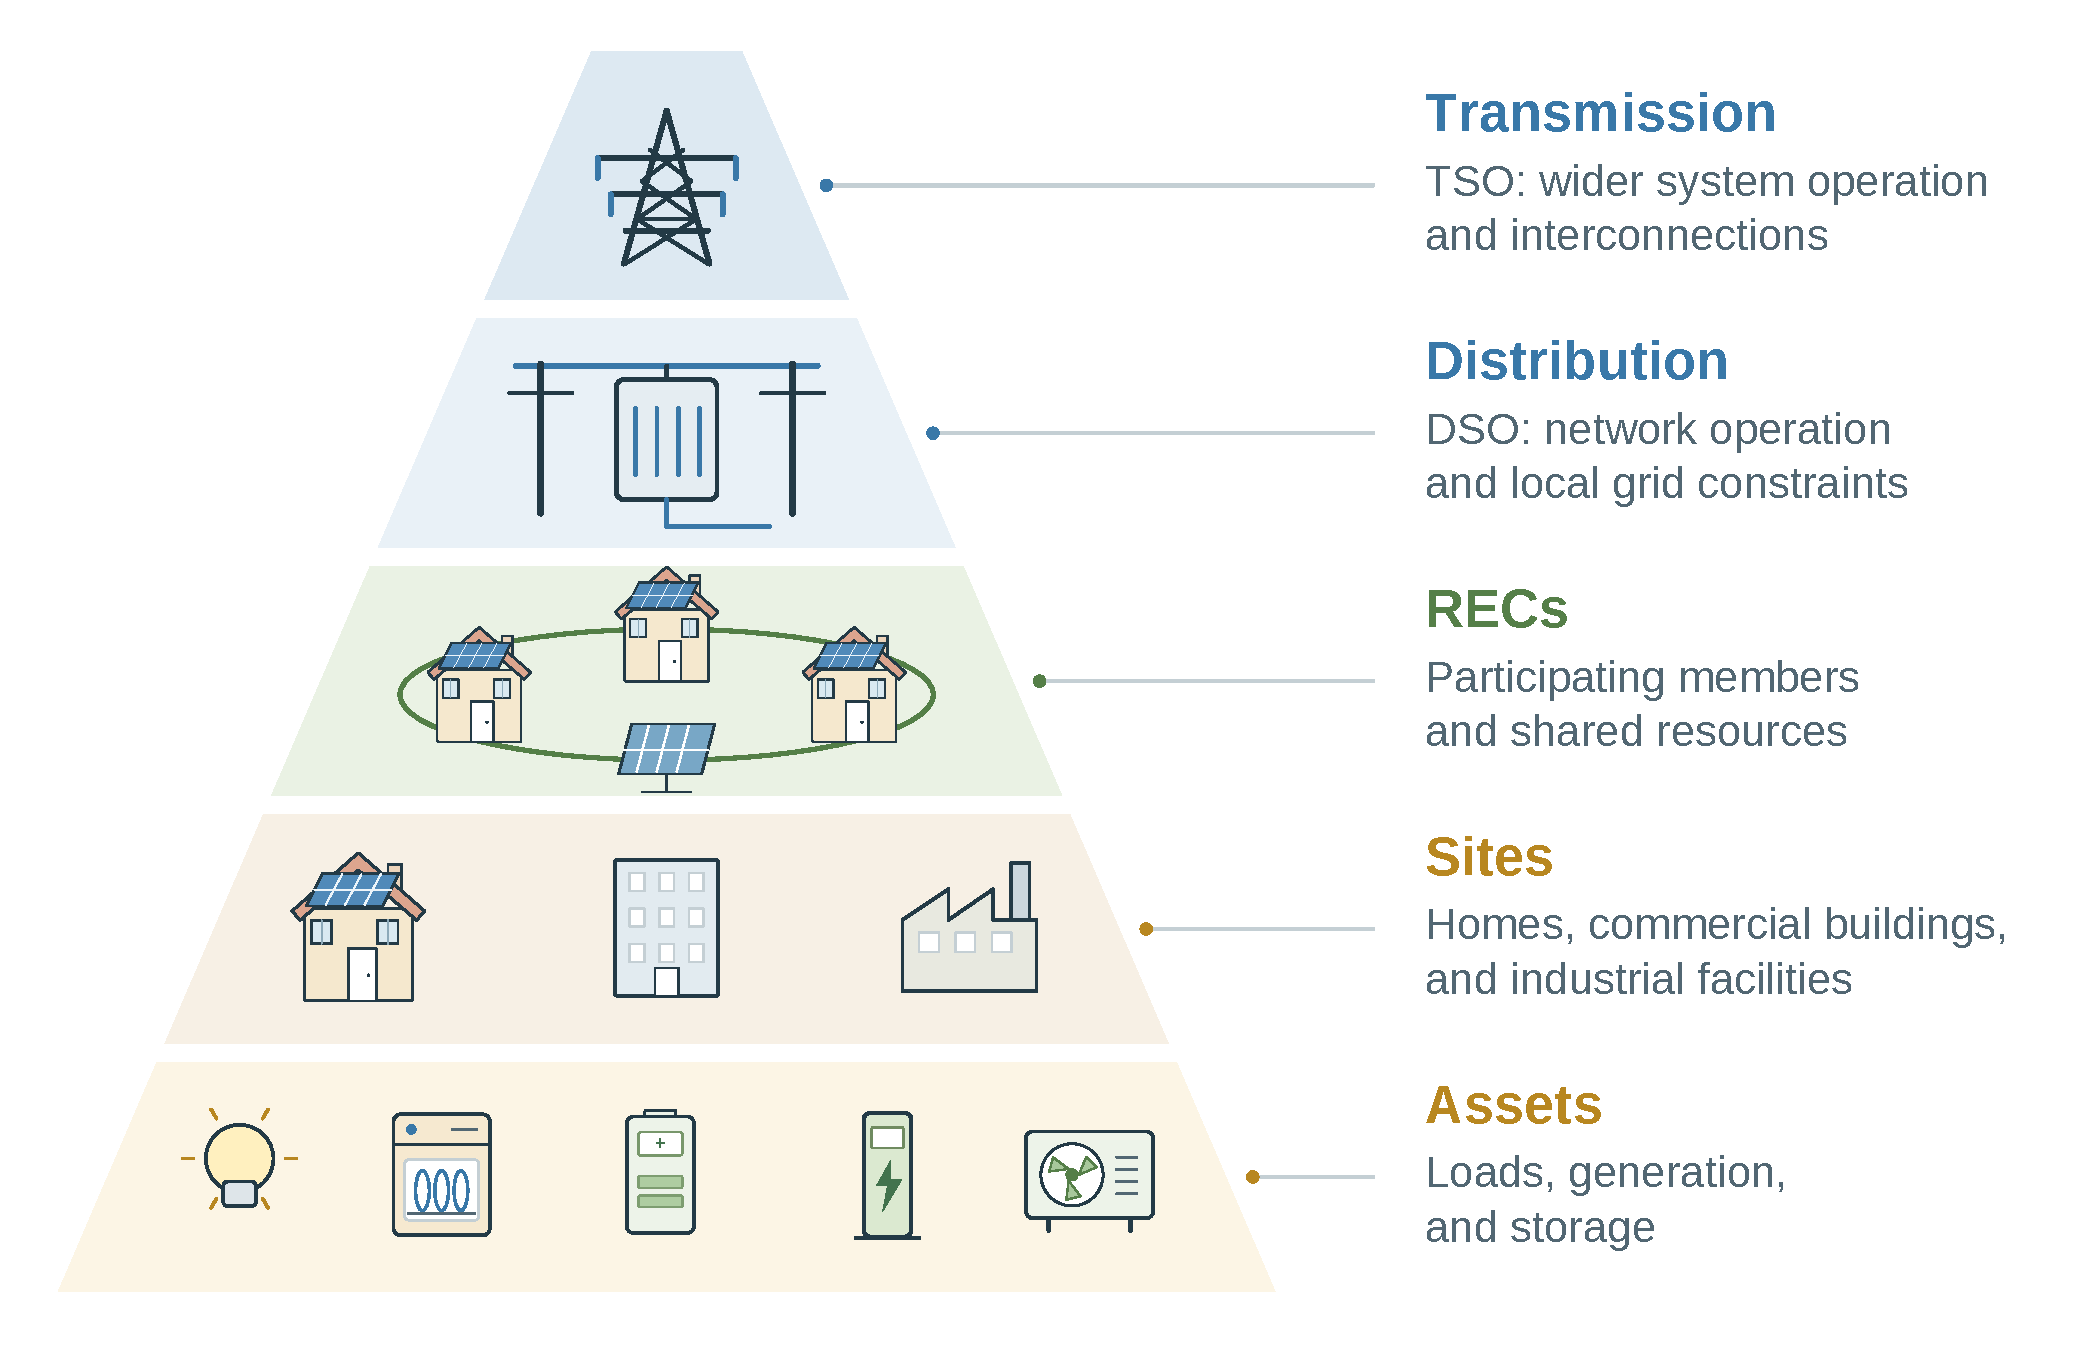
\includegraphics[width=\textwidth]{foundations-community-structure.pdf}
% Author-requested reminder: revise this illustration in a later visual pass.
\captionsetup{labelformat=reviewfigure}
\caption[Levels of organisation around a \gls{rec}]{Levels of organisation and coordination around a \gls{rec}. The pyramid relates assets and sites to \gls{rec} activities and the wider network context; membership arrangements and electrical connections determine the relationships in each installation.}
\label{fig:ch2-community-structure}
\end{figure}

Each level has its own \emph{operating limits}. An individual asset has technical limits associated with its physical design. For example, a charger can supply power within its rated range, and a battery can retain energy within its usable capacity. These limits describe the operation that the asset can support. Service requirements add conditions on its use, such as the energy a vehicle needs for departure or the temperatures occupants require in a room \parencite{hussain2023flexibility}.

At a site, several assets may share a \emph{single-phase} or \emph{three-phase} grid connection \parencite{eredes2025connectionmanual}. The power that can be supplied depends on the connection rating and the current limits of its conductors and protective devices. In a three-phase installation, the loading of each phase also matters, since one phase may reach its limit while capacity remains available on the others. The combined demand must respect these shared limits, even when each asset remains within its own rating. A charger and a heat pump, for example, may each operate at an admissible power while their simultaneous demand exceeds the capacity available to the home.

Similar relationships arise across sites connected to a common feeder or transformer. The scope of a shared electrical limit therefore follows the physical network connections, while \gls{rec} membership identifies the participants whose activities are coordinated.

Within these operating conditions, energy management can pursue objectives at each level. Table~\ref{tab:ch2-objectives-levels} summarises examples of these objectives and the conditions to preserve at each level.

\begin{table}[!htbp]
\centering\small
\caption[Energy-management objectives at different organisational levels]{Examples of energy-management objectives and operating conditions at different levels, synthesised from \textcite{hussain2023flexibility,moret2019energycollectives,reis2021businessmodels,eu2019electricity}.}
\label{tab:ch2-objectives-levels}
\renewcommand{\arraystretch}{1.16}
\begin{tabularx}{\textwidth}{@{}>{\RaggedRight\arraybackslash}p{0.16\textwidth}>{\RaggedRight\arraybackslash}X>{\RaggedRight\arraybackslash}X@{}}
\toprule
\textbf{Level} & \textbf{Examples of objectives} & \textbf{Conditions to preserve}\\\midrule
Asset & Reduce energy losses or wear during operation. & Technical limits and requested service, such as departure energy or thermal comfort.\\\addlinespace[6pt]
Site & Reduce expenditure and peak demand; increase local self-consumption. & Connection capacity and the service requirements of the site's assets.\\\addlinespace[6pt]
\gls{rec} & Increase shared use of renewable production; reduce collective expenditure; distribute benefits fairly. & Members' agreed requirements and applicable shared electrical limits.\\\addlinespace[6pt]
Distribution (\gls{dso}) & Reduce network losses; use network capacity efficiently. & Voltage and loading limits, with continuity of supply.\\\addlinespace[6pt]
Transmission (\gls{tso}) & Operate the wider system efficiently and coordinate exchanges between networks. & Supply--demand balance, frequency, and secure network operation.\\
\bottomrule
\end{tabularx}
\end{table}

\Needspace{3\baselineskip}
Asset characteristics and required services determine the operation available to meet these objectives. The next subsection explains how they define energy flexibility.

\Needspace{7\baselineskip}
\subsection{Asset Operation and Flexibility}
\label{sec:ch2-rec-flexibility}

Assets perform different functions within a site. Appliances and heating equipment create demand, \gls{pv} panels supply electricity, and a stationary battery retains energy for later use. An \gls{ev} combines storage with a mobility requirement and is available to the installation only while connected. Consumption, production, and storage determine the site's exchanges with the grid and the opportunities to adjust its energy use \parencite{hussain2023flexibility,siksnys2019flexoffers}.

\emph{Power} describes the rate of energy transfer, usually expressed here in kilowatts (kW), whereas \emph{energy} describes the amount transferred over an interval, in kilowatt-hours (kWh). A charger operating at 3~kW for one hour transfers 3~kWh at its electrical input. Losses mean that the increase in stored battery energy can be smaller. A storage asset's energy capacity and power rating express separate limits: capacity determines how much it can hold, while the power rating limits how quickly it can charge or discharge. Its \gls{soc} expresses the stored energy relative to a stated reference capacity. These distinctions matter when a service specifies an energy target but the asset accepts a power command.

At the building boundary, \emph{import} is electricity drawn from the external network and \emph{export} is electricity supplied to it. Local generation can meet demand directly, charge storage, or be exported. \emph{Self-consumption} concerns the use of locally generated electricity within the accounting boundary being considered. That boundary may be a building or a \gls{rec}, and the treatment of storage must be stated when the quantity is measured. \gls{rec} sharing allocates locally produced energy among participating members under the applicable arrangement. The allocation is distinct from the physical paths taken by electricity through the network \parencite{moret2019energycollectives,reis2021businessmodels}. A \gls{rec}'s membership and the assets behind one constrained electrical connection can consequently define different groups.

The timing of these exchanges affects the loading of the installation. A \emph{power peak} is the highest power observed over a stated period, with its value depending on the measurement or averaging interval used. Starting the \gls{ev}'s charging while cooking and heating are already drawing power can raise the home's evening import peak. At \gls{rec} level, the peak of the combined demand depends on how closely consumption at different sites coincides.

\emph{Ramping} describes changes in power over time, and a \emph{ramp rate} expresses how quickly power increases or decreases. A charger starting at full power produces an upward change in demand; a gradual increase spreads that change over a longer interval. The size of a peak and the speed of a change describe different features of the same power profile. Adjusting when charging begins and how its power develops can influence both, subject to the energy needed for departure.

\emph{Energy flexibility} is the scope for changing consumption, production, storage, or exchange relative to a reference behaviour while preserving the required service. It depends on the adjustments that the asset permits, its availability, and the time remaining to deliver that service. In the example from Section~\ref{sec:intro-energy-flexibility}, the \gls{ev} arrives at 18:00 with 30\% \gls{soc} and is required to reach 80\% by 08:00. These fourteen hours define the period available to meet the charging request, while the charger's power rating limits how quickly energy can be delivered. The session may allow several hours of delay early in the evening, but much less as departure approaches. Even a controllable charger offers no charging flexibility while the \gls{ev} is absent \parencite{hussain2023flexibility,siksnys2019flexoffers}.

A \emph{FlexOffer} describes this scheduling freedom through an admissible start-time window and an energy profile divided into intervals \parencite{siksnys2019flexoffers,fonseca2022flexloads}. Figure~\ref{fig:ch2-flexoffer} illustrates the two choices: when the charging profile begins and how much energy is assigned to each interval.

\begin{figure}[!htbp]
\centering
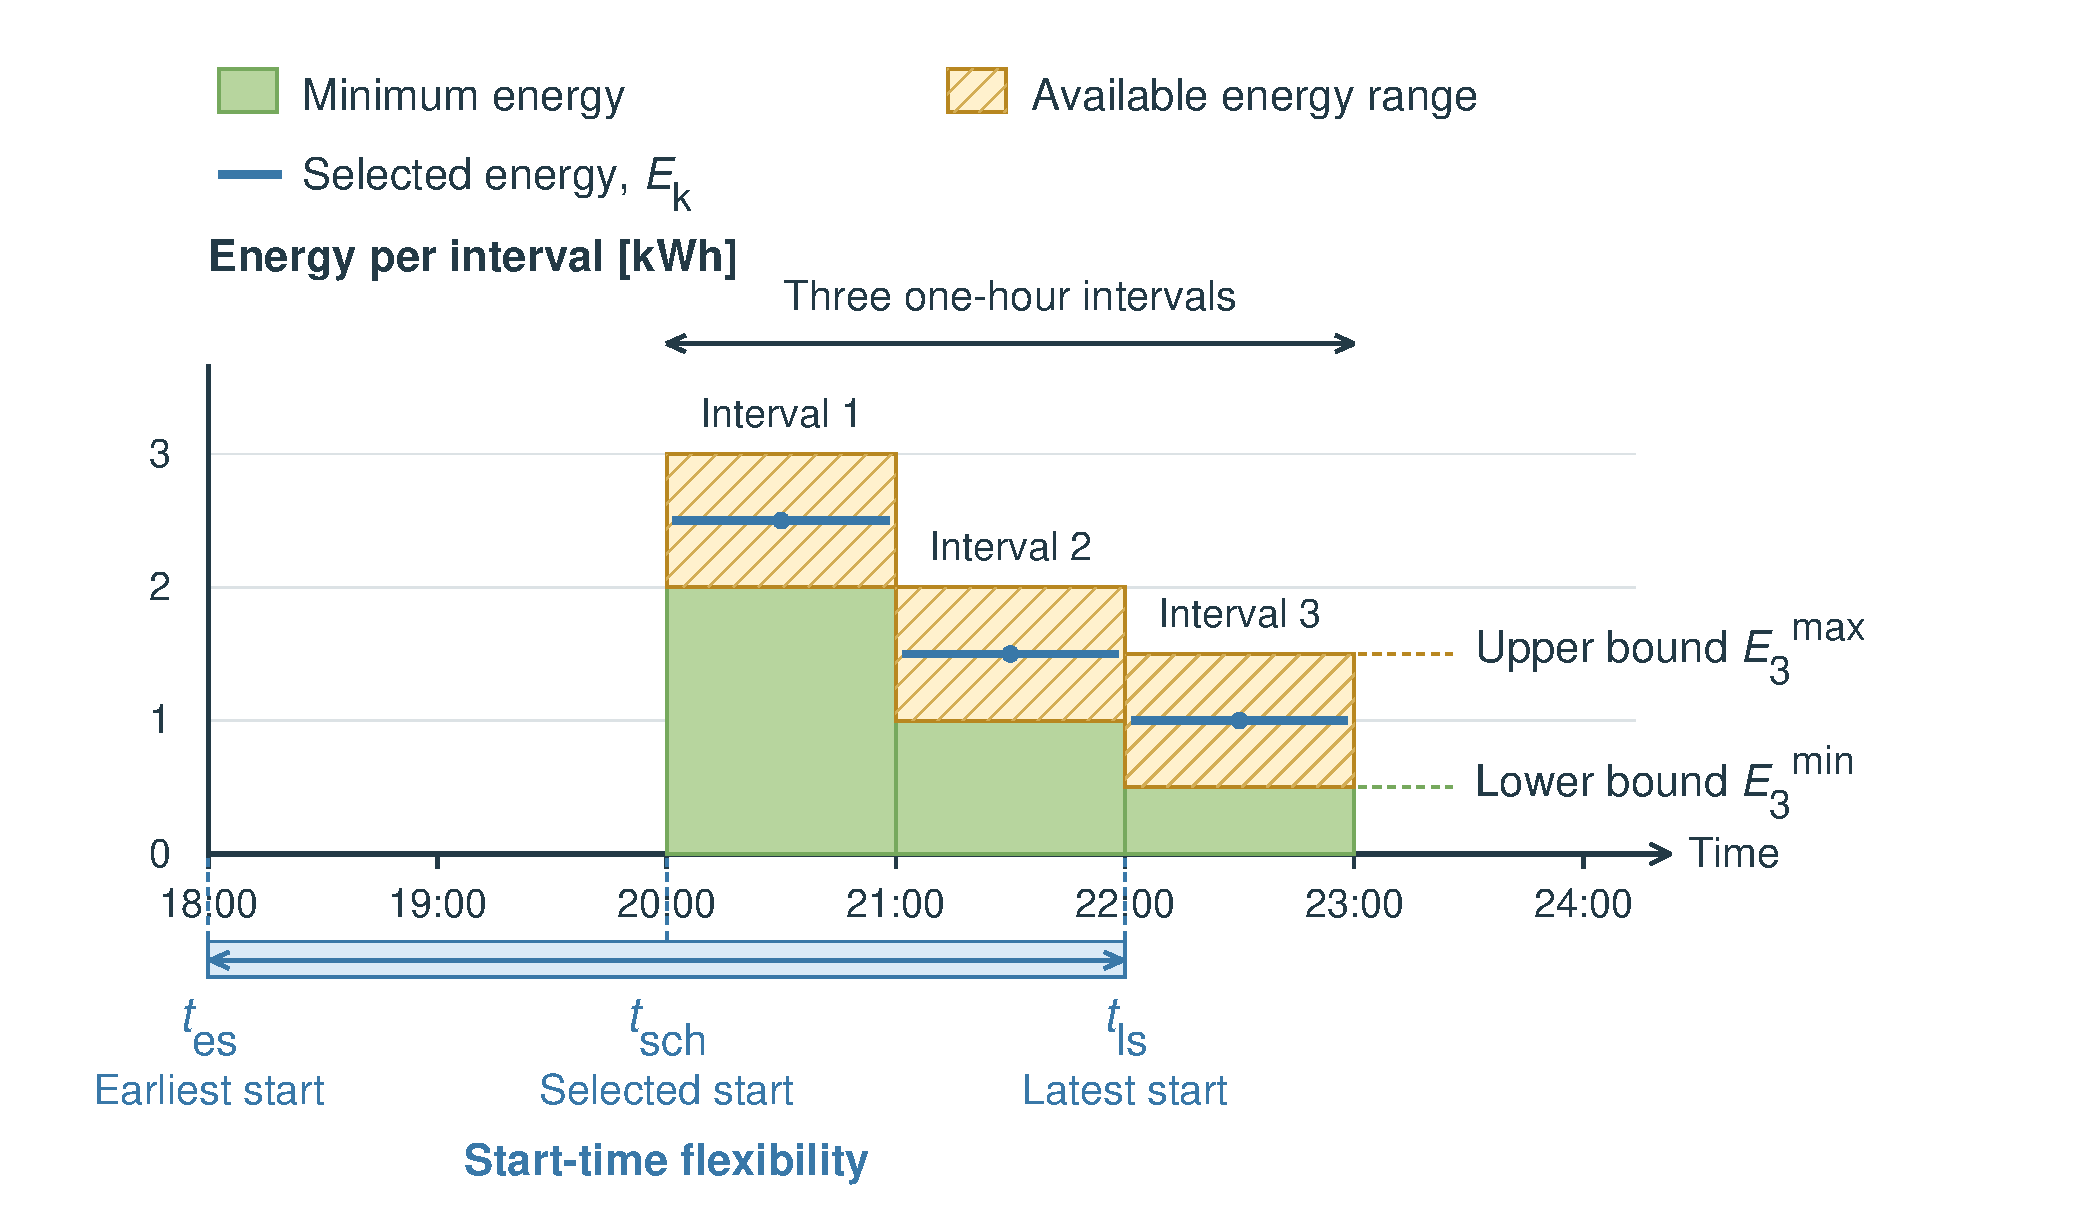
\includegraphics[width=0.90\textwidth]{foundations-flexoffer.pdf}
\caption[Start-time and energy flexibility in a FlexOffer]{Start-time and energy flexibility in a FlexOffer. Redrawn and adapted from \textcite{fonseca2022flexloads}; the values illustrate a profile rather than measured consumption.}
\label{fig:ch2-flexoffer}
\end{figure}

\Needspace{7\baselineskip}
For $N$ intervals of duration $\Delta t$, a FlexOffer $\mathcal F$ is written as:
\begin{equation}
\mathcal F=\left([t_{\mathrm{es}},t_{\mathrm{ls}}],
\left\langle [E_k^{\min},E_k^{\max}]\right\rangle_{k=1}^{N},\Delta t\right).
\label{eq:ch2-flexoffer}
\end{equation}
Here $t_{\mathrm{es}}$ and $t_{\mathrm{ls}}$ are the earliest and latest permitted start times. The ordered profile contains $N$ intervals, each with lower and upper energy bounds $E_k^{\min}$ and $E_k^{\max}$. The index $k$ identifies an interval relative to the profile's start, and $\Delta t$ specifies its duration.

Scheduling selects a start time $t_{\mathrm{sch}}$ and an energy amount $E_k$ for each interval, subject to:
\begin{equation}
t_{\mathrm{es}}\leq t_{\mathrm{sch}}\leq t_{\mathrm{ls}},
\qquad E_k^{\min}\leq E_k\leq E_k^{\max},
\quad k=1,\ldots,N.
\label{eq:ch2-flexoffer-schedule}
\end{equation}
The selected time $t_{\mathrm{sch}}$ positions the whole profile, while each $E_k$ fixes the energy transferred during its corresponding interval. Thus, the horizontal range in the figure represents a choice of start time, and the vertical ranges represent choices of energy. The profile lasts $N\Delta t$, so a service with deadline $t_{\mathrm{dep}}$ requires $t_{\mathrm{sch}}+N\Delta t\leq t_{\mathrm{dep}}$. The latest permitted start must leave enough time for that duration.

Lower and upper bounds on total energy, $E_{\mathrm{tot}}^{\min}$ and $E_{\mathrm{tot}}^{\max}$, couple the interval choices through:
\begin{equation}
E_{\mathrm{tot}}^{\min}\leq\sum_{k=1}^{N}E_k\leq E_{\mathrm{tot}}^{\max},
\label{eq:ch2-flexoffer-total}
\end{equation}
where $E_{\mathrm{tot}}^{\min}$ and $E_{\mathrm{tot}}^{\max}$ bound the energy transferred over the complete profile. An exact energy requirement $E_{\mathrm{req}}$ is represented by setting both bounds to $E_{\mathrm{req}}$. In \gls{ev} charging, this condition preserves the requested total while permitting energy to move between intervals. The target and interval bounds must refer to the same measurement boundary; a target expressed as stored battery energy must also account for charging losses. Together with the vehicle's availability, these conditions determine which schedules can deliver the service. Compatible offers can then be aggregated for scheduling and assigned back to individual assets \parencite{siksnys2019flexoffers}.

The flexibility available from an asset depends on which of these adjustments it supports. Figure~\ref{fig:ch2-resource-flexibility} illustrates fixed, shiftable, and elastic operation through household assets, including stationary storage.

\begin{figure}[!htbp]
\centering
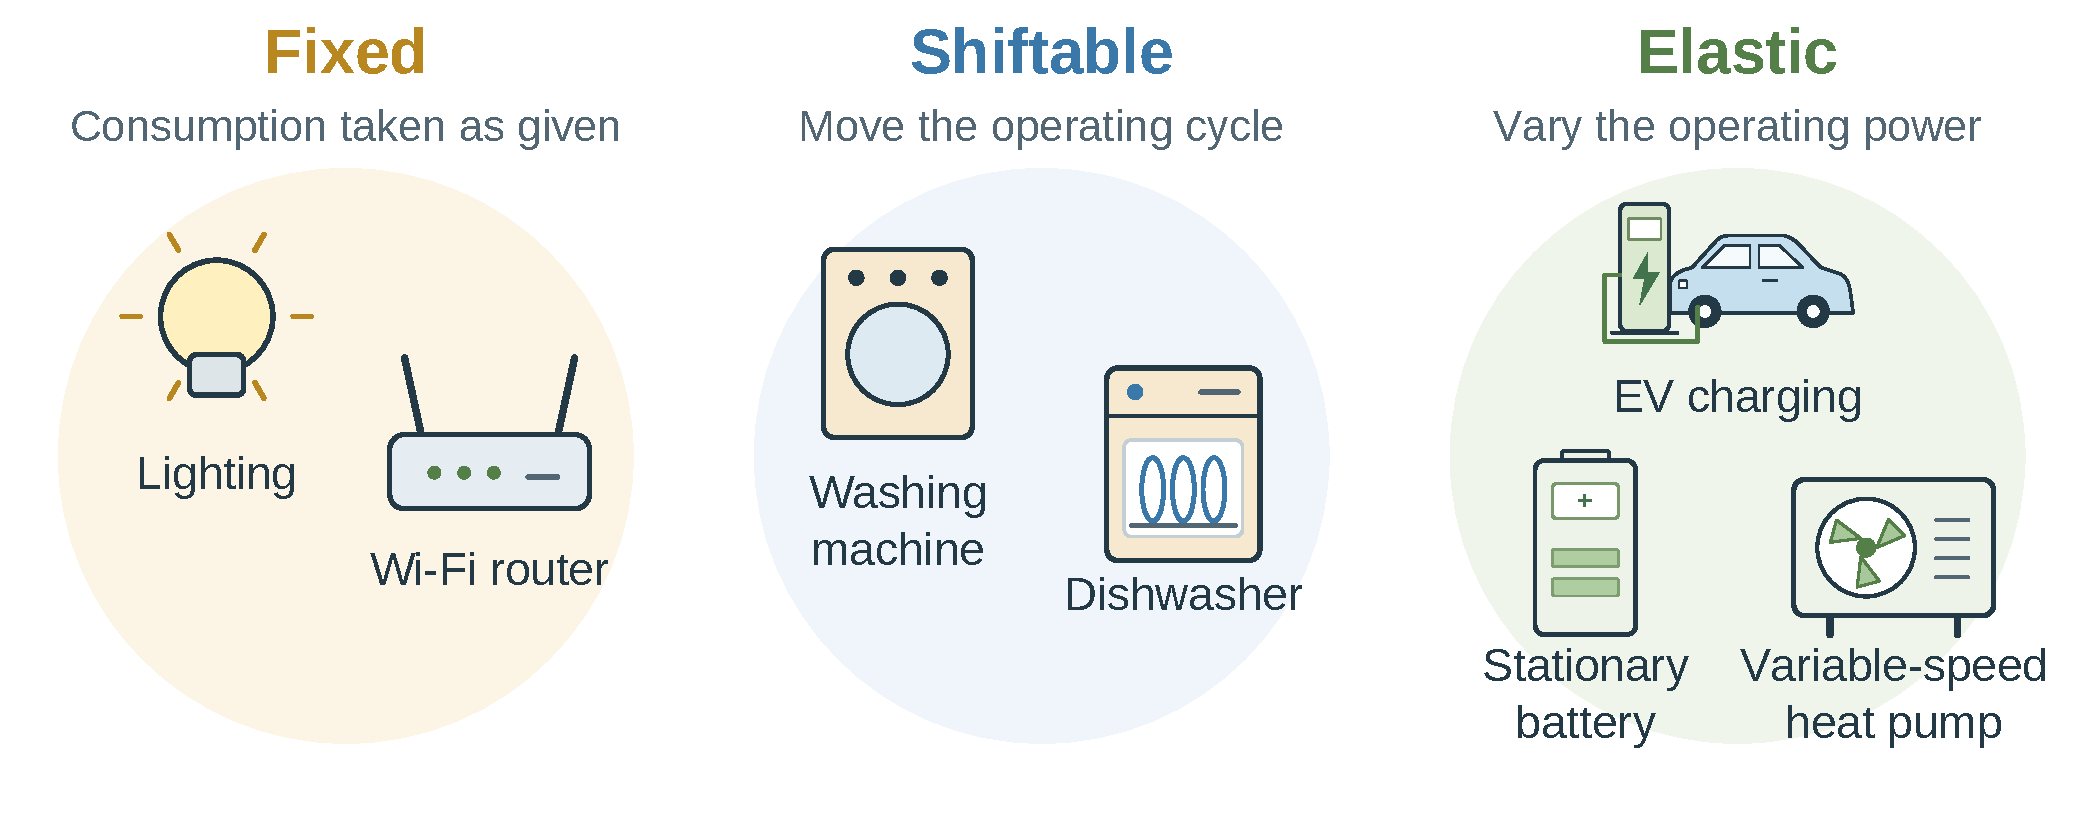
\includegraphics[width=\textwidth]{foundations-resources.pdf}
\caption[Fixed, shiftable, and elastic assets]{Household assets illustrating fixed, shiftable, and elastic operation. Stationary storage provides elastic operation through controllable charging and discharging.}
\label{fig:ch2-resource-flexibility}
\end{figure}

\Needspace{6\baselineskip}
\emph{Fixed} or non-shiftable loads, such as lighting required while a room is occupied, contribute \emph{non-controllable demand}: consumption taken as externally determined at the control timescale. Such demand can still be measured and included when scheduling controllable assets. In the FlexOffer description, a fixed profile has $t_{\mathrm{es}}=t_{\mathrm{sch}}=t_{\mathrm{ls}}$ and $E_k^{\min}=E_k=E_k^{\max}$ for every interval $k$. Both its timing and its energy amounts are therefore specified in advance.

A \emph{shiftable} appliance allows the start of a required operating cycle to move within a time window. A dishwasher loaded after dinner, for example, may begin at different times provided its cycle finishes by morning. Once started, the cycle may need to proceed without interruption. Its temporal flexibility is represented by $t_{\mathrm{es}}<t_{\mathrm{ls}}$, while $E_k^{\min}=E_k^{\max}$ retains the fixed cycle profile in each interval.

An \emph{elastic} or modulable load allows its power to vary within an operating range. An \gls{ev} charger may reduce power during an evening peak and increase it later, changing the interval energy amounts while retaining the departure target. Storage belongs to this category through its controllable charging and discharging power. A stationary battery, for example, can adjust its charging or discharging power within its power limits and usable energy range. This flexibility appears as $E_k^{\min}<E_k^{\max}$ in at least one interval, with Equation~\ref{eq:ch2-flexoffer-total} expressing any total-energy requirement. For storage, the admissible interval choices also depend on the energy retained from earlier decisions and on conversion losses. A fixed start time can coexist with variable energy amounts, while the possibility of pausing operation depends on the asset and service \parencite{fonseca2022flexloads,hussain2023flexibility,siksnys2019flexoffers}.

The schedules permitted by this flexibility can lead to different energy bills and emissions. Their evaluation therefore also depends on the market arrangements and external signals associated with the \gls{rec}'s electricity use.

\Needspace{7\baselineskip}
\subsection{Energy Markets and Decision Signals}
\label{sec:ch2-energy-markets}

\gls{rec} members can purchase electricity to meet their demand and sell production that is available for export, either through individual contracts or collective arrangements. Within the \gls{rec}, energy-sharing agreements can allocate local production among participants, while a \emph{local energy market} can organise transactions between buyers and sellers. These arrangements specify how exchanged energy is valued and how costs and revenues are distributed \parencite{moret2019energycollectives,reis2021businessmodels}.

An \emph{electricity tariff} specifies the prices and charges applied to consumption. A flat energy price applies the same unit rate throughout the day, while a \emph{time-of-use tariff} assigns different rates to predefined periods. Under a \emph{dynamic tariff}, the energy price follows variations in wholesale markets, such as the day-ahead market \parencite{ersetariffstructure,eu2019electricity}. The full bill may also include network charges, taxes, and fixed components.

Environmental information provides another basis for choosing when to use electricity. \emph{Carbon intensity} expresses the greenhouse-gas emissions attributed to a unit of electricity, commonly in grams of CO$_2$ equivalent per kWh. It varies as the generation mix and exchanges between electricity systems change. A production-based value describes generation within an area, while a consumption-based value also accounts for imported electricity. The geographical boundary, time interval, and emissions-accounting method give the signal its meaning when comparing schedules \parencite{electricitymapsmethodology,electricitymapscarbonintensity}.

Using these signals to guide asset operation requires information about the installation and its condition. The next subsection introduces how this information is acquired and the operational conditions that affect its use.


\Needspace{7\baselineskip}
\subsection{Information and Operational Conditions}
\label{sec:ch2-energy-information}

\emph{Data acquisition} obtains measurements and status information from the real-world installation through smart meters, sensors, and asset interfaces. These provide electricity readings, quantities such as room temperature, and operating states or diagnostics, with the measurement points determining which parts of the installation can be observed. Interfaces may also provide \emph{control capabilities}, such as setting charging power, while feedback indicates whether a command was accepted and what the asset delivered \parencite{gopstein2021smartgrid}.

The \emph{sampling interval} is the time between successive measurements, and the \emph{sampling frequency} is the number taken per unit of time. Acquisition, transmission, and storage can follow different schedules: a meter could sample every second, transmit a batch every minute, and retain quarter-hour aggregates, reducing data volume at the cost of temporal detail \parencite{kelly2015ukdale}.

A \emph{timestamp} identifies when a measurement or event occurred, while a separate reception time makes communication delays visible. Consistent clocks and time zones allow records from different assets to be aligned, and an aggregated energy value also needs the interval it covers \parencite{stouffer2023otsecurity}.

A \emph{forecast} estimates a future quantity from information available when it is issued; demand, \gls{pv} production, and weather forecasts may be produced locally or obtained from external services \parencite{nweye2025citylearnv2}. Each forecast needs an issue time and a \emph{forecast horizon}, identifying how far into the future it extends, while retaining successive versions makes it possible to recover the information available at an earlier decision.

\emph{Data quality} concerns the suitability of records for their intended use: \emph{freshness} describes how recent a value is, \emph{validity} concerns its expected format and physical interpretation, and \emph{completeness} concerns the presence of required records.

Table~\ref{tab:ch2-operational-conditions} distinguishes availability, health, dependencies, and degraded operation through the charging example \parencite{stouffer2023otsecurity}.

\begin{table}[!htbp]
\centering\small
\caption[Availability, health, dependencies, and degraded operation]{Operational concepts and their interpretation in the charging example.}
\label{tab:ch2-operational-conditions}
\renewcommand{\arraystretch}{1.16}
\begin{tabularx}{\textwidth}{@{}>{\RaggedRight\arraybackslash}p{0.21\textwidth}>{\RaggedRight\arraybackslash}X>{\RaggedRight\arraybackslash}X@{}}
\toprule
\textbf{Concept} & \textbf{Meaning} & \textbf{Charging example}\\\midrule
\emph{Availability} & Whether an asset can be used for a service at a given time. & The vehicle is connected and charging is authorised.\\\addlinespace[6pt]
\emph{Operational health} & Condition of an asset or supporting component relative to its intended function. & A charger fault reduces the power it can deliver.\\\addlinespace[6pt]
\emph{Operational\newline dependency} & An asset, component, or information source required by a function. & Charging adjusted to site headroom requires a site demand measurement.\\\addlinespace[6pt]
\emph{Degraded operation} & Continuation of a service with reduced capability or performance. & Charging continues under a local limit when demand-based adjustment is unavailable, where local protection supports this mode.\\
\bottomrule
\end{tabularx}
\end{table}

\Needspace{5\baselineskip}
The preceding subsections establish the resources, signals, and information available for \gls{rec} energy management. The next section introduces neural networks, explaining the computational models used to represent learned predictions and decisions before turning to \gls{rl}.

\FloatBarrier
\section{Neural Networks and Learned Representations}
\label{sec:ch2-neural}

The preceding section established the resources, signals, and operating conditions involved in \gls{rec} energy management. Neural networks provide one way to transform this information into predictions or decisions. This section introduces their basic computation and learned representations, preparing the policy and value models used in the \gls{rl} sections and the structured architectures developed in Section~\ref{sec:ch2-structured}.

A \emph{neural network} represents a function $f_\theta$ with learned parameters $\theta$. In the vector formulation used here, the input $x\in\mathbb R^{d_{\mathrm{in}}}$ and output $y=f_\theta(x)\in\mathbb R^{d_{\mathrm{out}}}$ are numerical vectors; $d_{\mathrm{in}}$ and $d_{\mathrm{out}}$ count their components. Measurements supply numerical features, while categories require a numerical encoding. For a charger, three input components might represent \gls{soc}, time until departure, and electricity price, with one output component representing a power request \parencite{goodfellow2016deep}.

A \emph{feed-forward network} passes information from input to output through successive transformations. A \gls{mlp} uses dense layers, in which each unit combines all components from the preceding layer. Between input and output, one or more \emph{hidden layers} compute intermediate numerical vectors.

\Needspace{6\baselineskip}
The transformation producing the vector $h^{(\ell)}$ at layer $\ell$ is:
\begin{equation}
h^{(\ell)}=\sigma_\ell\!\left(W^{(\ell)}h^{(\ell-1)}+b^{(\ell)}\right),
\qquad h^{(0)}=x,
\label{eq:ch2-neural-layer}
\end{equation}
where $W^{(\ell)}$ contains the learned weights, $b^{(\ell)}$ is a bias vector, and $\sigma_\ell$ is the layer's activation function. The weights combine the incoming values, the bias supplies an offset, and the activation transforms the result before it passes to the next layer.

Nonlinear activations allow stacked layers to represent nonlinear relationships. A \gls{relu}, for example, replaces negative values by zero and leaves non-negative values unchanged. Other common activations include the sigmoid, with outputs between zero and one, and the hyperbolic tangent, with outputs between $-1$ and $1$. These functions produce continuous values rather than binary on/off decisions \parencite{goodfellow2016deep}.

The output's interpretation depends on the task. A numerical output can specify a continuous quantity such as charging power. For a discrete choice, such as charge or wait, the network can produce a vector of scores; a softmax transformation converts them into probabilities, from which a choice is selected. Section~\ref{sec:ch2-modular-policies} returns to these action mappings.

A dense network is configured for a fixed number of input and output components. In the charging example, changing the \gls{soc} changes one of the three input values. Adding battery temperature would instead require a fourth input and a corresponding change to the network's input connections. Section~\ref{sec:ch2-structured} introduces ways to organise changing collections of resources, including padding, entity representations, and attention-based architectures.

Figure~\ref{fig:ch2-neural} follows the charging example through three input components, four hidden components, and one output. The four hidden values form a \emph{learned representation} of the input, computed inside the network and passed to its output layer. They combine the supplied features using learned parameters; each hidden value need not correspond to a named physical quantity.

\begin{figure}[!htbp]
\centering
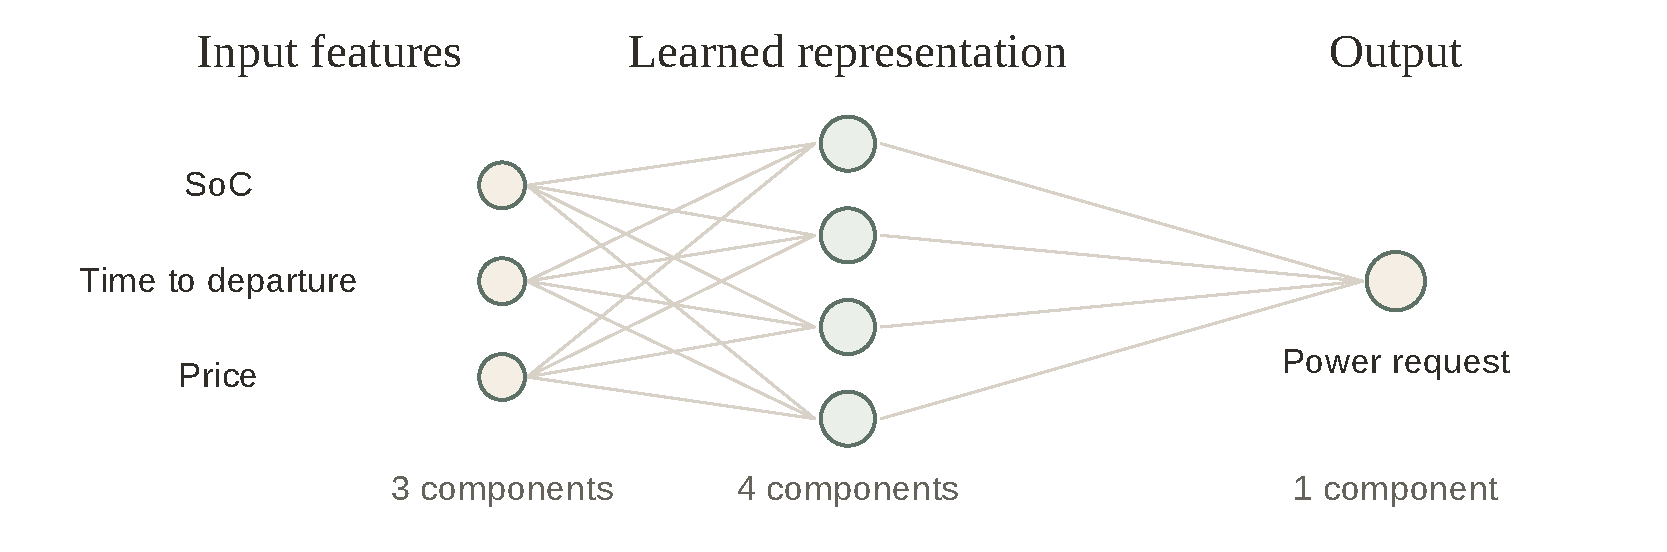
\includegraphics[width=\textwidth]{figures/foundations-neural.pdf}
\caption{A feed-forward network mapping three charging-related features through a learned representation to one output. The illustrated layer widths are architectural choices. Original illustration based on \textcite{goodfellow2016deep}.}
\label{fig:ch2-neural}
\end{figure}

\Needspace{3\baselineskip}
Such a representation is often called an \emph{embedding} when used as a numerical description for further computation. The part of the network that maps the inputs into this representation acts as an \emph{encoder}; a \emph{decoder} maps it into the required output. In the figure, the encoder produces the four hidden values and the decoder uses them to obtain the power request. Section~\ref{sec:ch2-structured} develops these roles for collections of resources.

Learning adjusts the parameters to minimise a \emph{loss function}. With known target outputs, the loss can measure the discrepancy between predictions and targets. \emph{Backpropagation} computes how the loss changes with the parameters, and an optimisation procedure uses these derivatives to update them \parencite{goodfellow2016deep}. Applying the trained network is \emph{inference}. During fixed-policy execution, new measurements produce new outputs while the parameters remain unchanged.

This section established how a network transforms numerical inputs into outputs and how its parameters are learned. The next section introduces \gls{rl}, where actions and their consequences supply the experience used to learn a decision rule.

\FloatBarrier
\Needspace{10\baselineskip}
\section{Reinforcement Learning}
\label{sec:ch2-rl}

\gls{rl} is based on the idea that a decision-maker can improve its choices by experiencing their consequences. Some \gls{rl} methods use the neural networks introduced in Section~\ref{sec:ch2-neural} to represent decision rules or estimates of future reward. This section introduces the foundations needed to understand the learning methods used in this thesis, covering the agent--environment interaction, the objective pursued over time, and the mechanisms used to learn a policy.

\Needspace{7\baselineskip}
\subsection{Sequential Decision-Making and Partial Observability}
\label{sec:ch2-mdp}
\label{sec:ch2-pomdp}

In sequential decision-making, an action can change both the immediate outcome and the choices available later. \gls{rl} represents this process as an interaction between an \emph{agent}, which selects actions, and an \emph{environment}, which responds to them.

\Needspace{7\baselineskip}
A \gls{mdp} $\mathcal M$ formalises this interaction \parencite{sutton2018rl}:
\begin{equation}
\mathcal M=(\mathcal S,\mathcal A,P,R,\gamma,\rho_0),
\label{eq:ch2-mdp}
\end{equation}
where $\mathcal S$ and $\mathcal A$ are the state and action spaces, $P(s'\mid s,a)$ is the transition distribution, and $R(s,a,s')$ is the expected immediate reward associated with a transition. The discount factor $\gamma$ determines the weighting of future rewards, and $\rho_0$ specifies the initial-state distribution.

At decision step $t$, the \emph{state} $s_t$ describes the conditions relevant to the task, and the \emph{action} $a_t$ specifies the agent's choice. The \emph{Markov property} means that $s_t$ summarises the information from past interactions needed to predict the next state $s_{t+1}$ and reward $r_t$, given $a_t$. Once $s_t$ and $a_t$ are known, the earlier sequence of states and actions adds no further information to that prediction. In the fully observable \gls{mdp} formulation, the agent has access to $s_t$ when choosing $a_t$ \parencite{sutton2018rl}.

A \emph{policy} $\pi$ determines how the agent selects $a_t$ from $s_t$. Applying $a_t$ leads to $s_{t+1}$ and a \emph{reward} $r_t$: a scalar signal that rates the outcome according to the task's objective, with larger values expressing more favourable outcomes. For a cost-minimisation objective, for example, the reward can be the negative cost incurred during the transition. Here $r_t$ denotes the signal received after $a_t$, while $R(s,a,s')$ gives its expected value for a specified transition \parencite{sutton2018rl}. Figure~\ref{fig:ch2-rl-cycle} illustrates this cycle, with $s_{t+1}$ providing the information for the next decision.

\begin{figure}[!htbp]
\centering
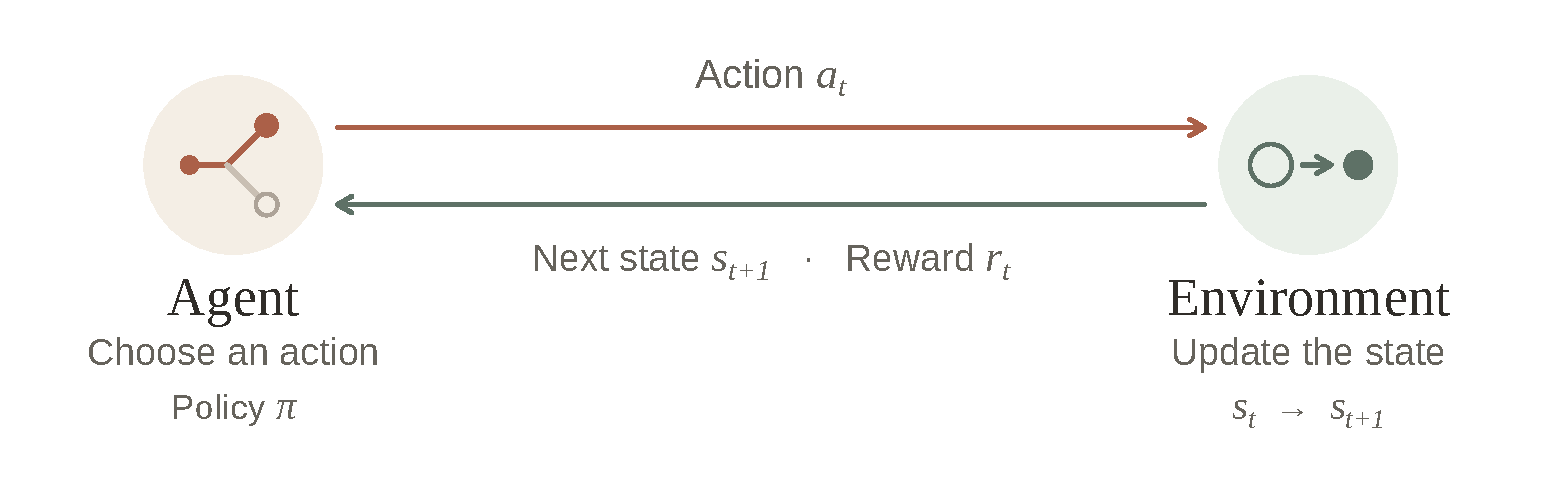
\includegraphics[width=0.86\textwidth]{figures/foundations-rl-cycle.pdf}
\caption{Agent--environment interaction in a fully observable \gls{mdp}. The reward $r_t$ follows action $a_t$, and the next state $s_{t+1}$ becomes available to the agent. Original illustration based on the formulation of \textcite{sutton2018rl}.}
\label{fig:ch2-rl-cycle}
\end{figure}

\gls{ev} charging illustrates this formulation within a \gls{rec}. The agent controls charging at a site (for example, a household), while the environment includes the vehicle, charger, and the site's electrical installation. The state $s_t$ includes the stored energy, departure target, time remaining, and relevant electrical conditions; $a_t$ is the selected charging power. Including the remaining time distinguishes the same battery \gls{soc} early in the evening from that \gls{soc} shortly before departure. Charging increases the stored energy as the remaining time decreases, producing $s_{t+1}$, while $r_t$ can reflect the cost of the energy delivered during the interval.

\Needspace{3\baselineskip}
In a real-world installation, the measurements available through sensors and interfaces determine which conditions the agent can observe, with noise or delays introducing further uncertainty \parencite{dulacarnold2021realworld}. The agent receives an \emph{observation} $o_t$ containing the available information about $s_t$. The task is \emph{partially observable} when this information provides an incomplete or uncertain description of the state relevant to its decisions, leaving some conditions affecting the outcome hidden from the agent.

\Needspace{7\baselineskip}
A \gls{pomdp} $\mathcal M_{\mathrm{PO}}$ extends the \gls{mdp} with an observation space and an observation model \parencite{kaelbling1998pomdp}:
\begin{equation}
\mathcal M_{\mathrm{PO}}=(\mathcal S,\mathcal A,P,R,\mathcal O,Z,\gamma,\rho_0),
\label{eq:ch2-pomdp}
\end{equation}
where $\mathcal O$ is the space of observations $o_t$ and $Z(o_{t+1}\mid s_{t+1},a_t)$ describes the distribution of the next observation after action $a_t$ leads to state $s_{t+1}$. The remaining components retain their \gls{mdp} meanings. The observation model describes how information about the underlying state becomes available to the agent.

For the charging agent, $o_t$ might contain measured charging power and the reported departure time while omitting battery \gls{soc}. The agent can observe the rate of energy delivery, but the energy already stored remains hidden, leaving uncertainty about how much more charging is needed. The interaction still follows the cycle in Figure~\ref{fig:ch2-rl-cycle}, with $o_{t+1}$ replacing direct access to $s_{t+1}$; the agent can use past observations and actions to help infer the missing state information.

A \emph{belief state} summarises this history as a probability distribution over possible states $s_t$, updated as actions are taken and new observations arrive. Given the \gls{pomdp} model and an initial belief, it provides sufficient information for selecting actions, although exact updates can be computationally demanding \parencite{kaelbling1998pomdp}. Practical policies can instead retain a window of past observations or use recurrent memory to integrate information over time \parencite{hausknecht2015drqn}.

The next subsection explains how the rewards received across successive decisions are combined into a return, and how value functions use that return to assess a policy over the course of a task, including consequences that only emerge after several actions.

\Needspace{7\baselineskip}
\subsection{Returns, Episodes, Value Functions, and Policies}
\label{sec:ch2-return-value}

In the interaction described above, the agent receives a reward $r_t$ after applying action $a_t$, giving feedback on that transition. Evaluating the policy requires following the consequences of successive choices, which the \emph{return} $G_t$ captures by accumulating rewards over the remainder of an episode or, for a continuing task, over a longer horizon.

An \emph{episode} groups successive interactions over a defined period. In a \gls{rec}, this may cover a day or a year of chronological data, containing many charging sessions and other asset operations. Lowercase $t$ indexes a decision step, while uppercase $T$ marks the end of the sequence, after the last action at $T-1$. A \emph{terminal state} marks the end of the modelled task; a selected data window can also end while the real-world operation continues.

\Needspace{7\baselineskip}
Over an episode ending at $T$, the discounted return $G_t$ from step $t$ combines the previously introduced rewards $r_t$ as:
\begin{equation}
G_t=\sum_{k=0}^{T-t-1}\gamma^k r_{t+k}.
\label{eq:ch2-return}
\end{equation}
Here $r_{t+k}$ is the reward received $k$ steps after $t$, weighted by $\gamma^k$, and the sum ends at the last transition before $T$. Continuing tasks can use an infinite discounted sum with $0\leq\gamma<1$, or an average-reward formulation. In finite tasks, $\gamma=1$ retains equal weight for rewards throughout the remaining episode when the return is well defined \parencite{sutton2018rl}.

If charging rewards are simply negative electricity costs and $\gamma=1$, $G_t$ is the negative total cost from the current step to the end of the episode. A discount factor below one reduces the contribution of distant rewards, with its effect depending on the decision interval. The same numerical value produces a different effective time horizon at one-minute and one-hour resolution.

\Needspace{6\baselineskip}
A stochastic policy $\pi(a\mid s)$ gives a distribution over actions; a deterministic policy $\mu(s)$ selects one action. The \emph{state-value function} $V^\pi(s)$ and \emph{action-value function} $Q^\pi(s,a)$ describe expected returns under $\pi$:
\begin{align}
V^\pi(s)&=\mathbb E_\pi[G_t\mid s_t=s],\\
Q^\pi(s,a)&=\mathbb E_\pi[G_t\mid s_t=s,a_t=a].
\label{eq:ch2-value-functions}
\end{align}
Here $\mathbb E_\pi$ denotes expectation under policy $\pi$, conditional on the current state $s$ or state--action pair $(s,a)$. It accounts for transitions and, where applicable, policy randomness. For finite-horizon problems these functions can depend on the remaining time; the notation suppresses this dependence when time is included in the state. For the \gls{ev}, $V^\pi(s)$ estimates the return from following the charging policy from the current conditions, while $Q^\pi(s,a)$ estimates the return from first choosing a particular charging power and then following that policy.

The Bellman relation expresses $Q^\pi(s,a)$ through the reward obtained now and the value of what follows:
\begin{equation}
Q^\pi(s,a)=\mathbb E\!\left[r_t+\gamma
\mathbb E_{a'\sim\pi(\cdot\mid s_{t+1})}Q^\pi(s_{t+1},a')
\mid s_t=s,a_t=a\right].
\label{eq:ch2-bellman}
\end{equation}
The outer expectation averages over the resulting reward $r_t$ and next state $s_{t+1}$; the inner expectation averages over the next action $a'$ drawn from $\pi$. At a terminal transition, the continuation value is zero. This recursion allows observed rewards and estimated future values to inform the same learning update. If the charging reward includes a penalty for energy missing at departure, an action with a small immediate cost can have a poor value because it leaves insufficient time to complete the service. The value function carries that later consequence into the present decision through the specified reward.

The \emph{advantage} $A^\pi(s,a)=Q^\pi(s,a)-V^\pi(s)$ compares an action with the policy's expected performance at the same state. For the \gls{ev}, a positive advantage means that the selected charging power has a higher expected return than the policy achieves on average from those conditions. This relative learning signal can reduce variability when updating a policy.

These comparisons depend on what the reward treats as a favourable outcome, which leads to the next subsection's question of how to construct that signal from the task's objectives.

\Needspace{7\baselineskip}
\subsection{Reward Design and Objective Specification}
\label{sec:ch2-reward}

The preceding subsection accumulated rewards into a return and used expected returns to evaluate a policy. The next step is to specify the reward function $R$ introduced in the \gls{mdp}, which determines what each transition contributes to that evaluation. In a \gls{rec}, this means translating objectives such as reducing expenditure, delivering the requested departure energy, and maintaining thermal comfort into the learning signal. These objectives were introduced at the asset, site, and \gls{rec} levels in Section~\ref{sec:ch2-rec-members} and Table~\ref{tab:ch2-objectives-levels}.

\Needspace{7\baselineskip}
Several such objectives can contribute to a single \emph{composite reward} $r_t$ through a weighted sum \parencite{roijers2013multiobjective}:
\begin{equation}
r_t=\sum_{j=1}^{m} w_j f_j(s_t,a_t,s_{t+1}),
\label{eq:ch2-composite-reward}
\end{equation}
where $m$ is the number of components, $f_j$ is the signal for outcome $j$, and $w_j\geq 0$ sets its weight. Each $f_j$ is expressed so that larger values are preferred; costs and shortfalls can therefore enter as negative terms. The components can conflict. Postponing \gls{ev} charging may reduce expenditure while increasing the energy missing at departure, so a gain in one term can be offset by a loss in another. The weights express the relative importance of these outcomes in the combined signal.

The numerical scale of each $f_j$ also affects this balance. For components measured in euros and kWh, the weights must account for both their numerical ranges and their intended relative importance. Normalisation can provide a reference scale, while changing either that scale or the weights changes the trade-off.

A service requirement can enter both the reward and the constraints governing the decision. A departure-energy penalty encourages learning to value readiness, while a constraint can require a charging schedule to deliver the requested energy whenever the available time and capacity permit. Electrical limits likewise restrict admissible actions. Reward terms guide the preference among outcomes; enforcing a requirement needs a mechanism that restricts the decisions applied, as introduced in Section~\ref{sec:ch2-constrained-foundations}.

Reward design also determines when feedback is supplied. A \emph{sparse} reward occurs only at selected events, such as task completion or failure, whereas a \emph{dense} reward provides more frequent feedback throughout the interaction. Sparse feedback can express the final outcome directly, although identifying which earlier decisions contributed to it becomes more difficult. In the charging example, expenditure may contribute at every interval while readiness is assessed at each departure within the episode; discounting then affects the relative influence of these contributions. Dense feedback can help learning recognise progress, but rewarding an intermediate quantity may favour behaviour that improves that quantity while weakening the final outcome \parencite{sutton2018rl}.

\Needspace{8\baselineskip}
\emph{Reward shaping} supplies additional feedback during learning to make useful intermediate progress easier to recognise. For an \gls{ev}, this can help relate successive charging decisions to the energy needed at departure, before that service is finally assessed. In potential-based shaping, a function $\Phi$ assigns a numerical measure of progress to each state and defines a shaped reward $r_t^{\Phi}$ \parencite{ng1999shaping}:
\begin{equation}
r_t^{\Phi}=r_t+\gamma\Phi(s_{t+1})-\Phi(s_t).
\label{eq:ch2-potential-shaping}
\end{equation}
Here $\Phi(s_t)$ and $\Phi(s_{t+1})$ evaluate the current and next states, and $\gamma$ is the discount factor already used in the return. Their discounted difference is added to the original reward $r_t$. In the charging example, $\Phi$ could assign higher values as the energy shortfall decreases, providing feedback about progress between successive decisions.

The reward function now specifies the feedback available to the learning process, while the return combines that feedback over time. The next subsection explains how experience from successive interactions is used to estimate values and improve the policy.

\Needspace{7\baselineskip}
\subsection{Learning from Experience}
\label{sec:ch2-experience}
\label{sec:ch2-policy-gradient}

Learning uses the feedback defined above to improve subsequent decisions. Each interaction records the conditions faced by the agent, the action it applied, and the resulting reward and next state. In the \gls{rec} example, a charging decision reveals how the selected power affects stored energy, electricity expenditure, and the time remaining to meet the departure target.

\emph{Value-based learning} estimates the return associated with states or actions and uses those estimates to choose decisions. For the charging agent, this means learning how promising charging now, waiting, or selecting a lower power is from the current conditions, considering their consequences through the rest of the episode. Experience revises these estimates, helping the agent choose actions with higher expected return \parencite{sutton2018rl,watkins1992qlearning}.

\Needspace{8\baselineskip}
\emph{Policy-based learning} adjusts the rule that selects actions. For example, the charging agent can learn to assign a higher probability to power settings that perform better than expected in the conditions it encounters. The parameters $\theta$ control this rule, represented by a differentiable policy $\pi_\theta$. The policy-gradient principle relates an improvement in expected return to terms of the form:
\begin{equation}
\mathbb E\!\left[\nabla_\theta\log\pi_\theta(a_t\mid s_t)
A^{\pi_\theta}(s_t,a_t)\right],
\label{eq:ch2-policy-gradient}
\end{equation}
where $\nabla_\theta$ differentiates with respect to the policy parameters, $\log\pi_\theta$ is the log-probability of the selected action, and $A^{\pi_\theta}$ is its advantage. The expectation averages over the states and actions used by the method. The advantage guides the update towards making better-than-expected actions more likely and worse-than-expected actions less likely in comparable conditions \parencite{sutton1999policygradient}.

An \emph{actor--critic} method brings these two roles together. The actor selects an action, while the critic estimates the values used to assess it and guide learning. In the \gls{rec} example, the actor chooses charging power and the critic helps judge whether that choice improves the expected return.

\emph{Exploration} allows the agent to learn about alternatives to its current preferred action. A charging agent might try two permitted power levels in similar conditions to learn how their consequences differ. A stochastic policy can sample different actions, while a deterministic policy can use a perturbation during experience collection. In a real-world installation, these choices must respect the available operating limits.

\emph{Entropy regularisation} encourages a stochastic policy to retain variety in its action choices while improving return. For the charging agent, this can help avoid concentrating too early on a single power setting. Its coefficient controls the strength of that encouragement \parencite{haarnoja2018sac}.

\emph{On-policy} and \emph{off-policy} learning describe how the policy that collects experience relates to the one being learned. An on-policy charging agent learns from decisions made with the policy currently being improved. An off-policy method can also learn from decisions made by an earlier or different controller. The distinction identifies which policy generated the data; online and offline learning instead distinguish whether new interactions are collected during learning.

A \emph{replay buffer} stores transitions so that an off-policy method can reuse them in later updates. A recorded charging decision can therefore contribute to learning more than once, even after the controller has changed. Learning entirely from a fixed archive is developed in Section~\ref{sec:ch2-offline}.

Building on the learning methods described above, the next subsection explains how knowledge from an existing controller can help the agent learn useful behaviour, and how operational constraints govern the choices it can apply during learning and subsequent operation.

\Needspace{7\baselineskip}
\subsection{Prior Knowledge and Constrained Decisions}
\label{sec:ch2-constrained-foundations}

The learning process described above can begin with knowledge of how the installation is already operated. In a \gls{rec}, a \gls{rbc} may already schedule charging using electricity prices, battery \gls{soc}, and departure requirements. This \emph{prior knowledge} can help the agent learn useful behaviour through examples, guidance during exploration, or adjustments to an existing control rule.

\emph{\gls{bc}} learns to reproduce a controller's or expert's decisions from demonstrations that pair the conditions encountered with the actions chosen. For the charging agent, these examples associate the vehicle's needs and the electricity price with a selected charging power. Supervised learning fits the policy to these choices; when rewards and subsequent states are also recorded, the transitions can support \gls{rl} \parencite{ross2011dagger}.

\emph{Guided exploration} uses existing knowledge to direct the agent towards promising actions while collecting experience. A controller's recommended charging power, for example, can provide a starting point for trying nearby permitted power levels. The resulting rewards and state changes then inform the learner's own decisions.

\emph{Residual learning} retains the existing controller as part of the decision rule and learns an adjustment to its output. In the charging example, the controller supplies a reference power and the learned policy increases or decreases that value in response to the current conditions \parencite{johannink2019residual}.

These ways of using prior knowledge operate within the installation's physical and service requirements. \emph{Constraints} express which actions or sequences of actions are admissible. A constrained \gls{mdp} can maximise expected reward subject to budgets $d_j$ on expected accumulated costs $c_j$, written generically as:
\begin{equation}
\mathbb E_\pi\!\left[\sum_t\gamma^t c_j(s_t,a_t)\right]\leq d_j,
\qquad j=1,\ldots,m,
\label{eq:ch2-cmdp}
\end{equation}
where $j$ indexes the $m$ constraints, $c_j(s_t,a_t)$ is the cost at step $t$, and $d_j$ is its permitted accumulated budget. The expectation averages discounted costs over trajectories generated by $\pi$ \parencite{achiam2017cpo}. Such a condition concerns an expectation over trajectories. An instantaneous equipment limit instead applies to every relevant command, and a deadline condition depends on a sequence of decisions. These meanings require different enforcement mechanisms.

An action mask can remove inadmissible discrete choices before selection. For continuous decisions, a projection or safety filter can map a proposed action into an admissible set determined by a constraint model. A supervisory controller may supply a fallback when the proposed decision cannot be used \parencite{dalal2018safe,elsayedaly2021shielding}.

This section introduced how an agent learns a policy from rewards and experience, with prior knowledge and constraints guiding its decisions. The next section extends these foundations to \gls{marl}, where agents interact within a shared environment such as a \gls{rec}.

\Needspace{8\baselineskip}
\FloatBarrier
\section{Multi-Agent Reinforcement Learning}
\label{sec:ch2-marl}

The preceding section considered how one agent learns to act on its environment. In \gls{marl}, several agents learn while their decisions jointly affect that environment. Consider a \gls{rec} in which each site has an agent controlling its \gls{ev} charging. If two agents charge during the same low-price period, their simultaneous charging can create a \gls{rec} demand peak. This section extends the decision model to such interactions, then explains how learning is organised and how individual decisions contribute to a shared outcome.

\Needspace{7\baselineskip}
\subsection{Markov Games and Multi-Agent Objectives}
\label{sec:ch2-markov-games}

The \gls{mdp} described one agent's action at each step. With several agents, the environment responds to their combined choices, represented by a \emph{joint action}. A Markov game $\mathcal G$, also called a stochastic game, expresses this interaction \parencite{shapley1953stochastic,littman1994markovgames}. A discounted formulation is:
\begin{equation}
\mathcal G=\left(\mathcal N,\mathcal S,
\{\mathcal A_i\}_{i\in\mathcal N},P,
\{R_i\}_{i\in\mathcal N},\gamma,\rho_0\right),
\label{eq:ch2-markov-game}
\end{equation}
where $\mathcal N=\{1,\ldots,n\}$ is the fixed agent set and $\mathcal A_i$ is agent $i$'s action space. The joint action $a=(a_1,\ldots,a_n)$ belongs to the product of those spaces. The transition distribution is now $P(s'\mid s,a)$, and each agent has an expected reward $R_i(s,a,s')$. As in the \gls{mdp}, $\mathcal S$ is the state space, $\gamma$ the discount factor, and $\rho_0$ the initial-state distribution.

In the \gls{rec} example, $a_{i,t}$ is the charging power selected at site $i$, and $a_t$ collects all sites' choices at that step. Their combined charging changes the vehicles' stored energy and the \gls{rec}'s total demand. Each agent's reward can therefore depend on both its own choice and the choices made elsewhere in the \gls{rec}.

A \emph{fully cooperative} game gives all agents the same reward and a common performance objective. For the charging agents, that reward could combine \gls{rec} electricity expenditure, peak demand, and the energy missing at vehicle departures. Each site's decisions then contribute to the outcome that all agents learn to improve.

A \emph{general-sum} game allows agents to have different rewards, expressing objectives that may partly coincide and partly conflict. In a \gls{rec}, members may pursue individual expenditure targets alongside a \gls{rec} objective. In a \emph{zero-sum} game, the agents' rewards sum to zero for every transition. With two agents, one agent's reward is therefore the negative of the other's \parencite{wang2022coopcompetitive,moret2019energycollectives}.

The community-control problem studied in this thesis assumes agreement on the collective objectives and individual service commitments to be considered. Reducing a community peak, for example, is pursued alongside the energy required by each vehicle at departure. These commitments enter the control formulation through constraints, reward terms, and assessment of the service delivered. Cooperation is therefore a choice in the formulation of the control problem. A common reward defines the fully cooperative case, while formulations combining local and community rewards retain agent-specific objectives whose effects on coordination must be assessed. Each controller's reward construction is specified in the corresponding method description. Assessing individual outcomes also remains necessary to establish how the benefits and burdens of coordination are distributed.

Under \emph{partial observability}, each agent receives an observation $o_{i,t}$ that does not necessarily reveal all the state information relevant to its decisions. The charging agent might observe its own vehicle's \gls{soc} and departure time together with a published electricity price. Its action can depend on its local history $h_{i,t}$ of observations and previous actions.

\Needspace{8\baselineskip}
The individual policies together define the joint policy $\pi$. When agents sample independently conditional on their local histories, it factorises as:
\begin{equation}
\pi(a_t\mid h_t)
=\prod_{i\in\mathcal N}\pi_i(a_{i,t}\mid h_{i,t}).
\label{eq:ch2-joint-policy}
\end{equation}
Here $a_t=(a_{1,t},\ldots,a_{n,t})$ and $h_t=(h_{1,t},\ldots,h_{n,t})$ collect the agents' actions and local histories, and $\pi_i$ is agent $i$'s policy. The product combines the probabilities of their individual choices into the probability of the joint action. In the example, each site's agent chooses a charging power from its available information, and those choices are applied together.

A \gls{decpomdp} formalises cooperation under a common reward, with agents acting from local observations and action histories \parencite{oliehoek2016decpomdp}.

\Needspace{7\baselineskip}
\subsection{Learning and Execution Organisation}
\label{sec:ch2-ctde}
\label{sec:ch2-parameter-sharing}

The joint policy can be learned and applied through different organisational arrangements. Learning determines which experience and information support policy updates, while execution determines how actions are selected in operation. Parameter sharing concerns whether several agents use the same learned decision rule.

\emph{Independent learning} lets each agent improve its policy while treating the other agents as part of the environment. In the \gls{rec} example, each site learns from its available observations, charging decisions, and rewards \parencite{tan1993independent,claus1998dynamics}.

\emph{Non-stationarity} arises from the other agents' changing behaviour during learning. If one site learns to move its charging to an earlier period, the \gls{rec} demand experienced by another site changes. The second agent is therefore learning while part of its environment is also adapting. Recorded experience can contain transitions from several stages of this adaptation \parencite{foerster2017replay}.

\emph{Centralised execution} selects the joint action through one decision process using combined information. A \gls{rec} controller could, for example, select all sites' charging powers together. With \emph{decentralised execution}, each site's agent selects its own action from its inputs, which can include local measurements and shared signals or messages.

\gls{ctde} uses joint information during learning while retaining local action selection in operation \parencite{lowe2017maddpg,albrecht2024marl}. Figure~\ref{fig:ch2-ctde} illustrates how a centralised critic supports policy updates during training, while each site's actor selects charging power from its available inputs during execution.

\begin{figure}[!htbp]
\centering
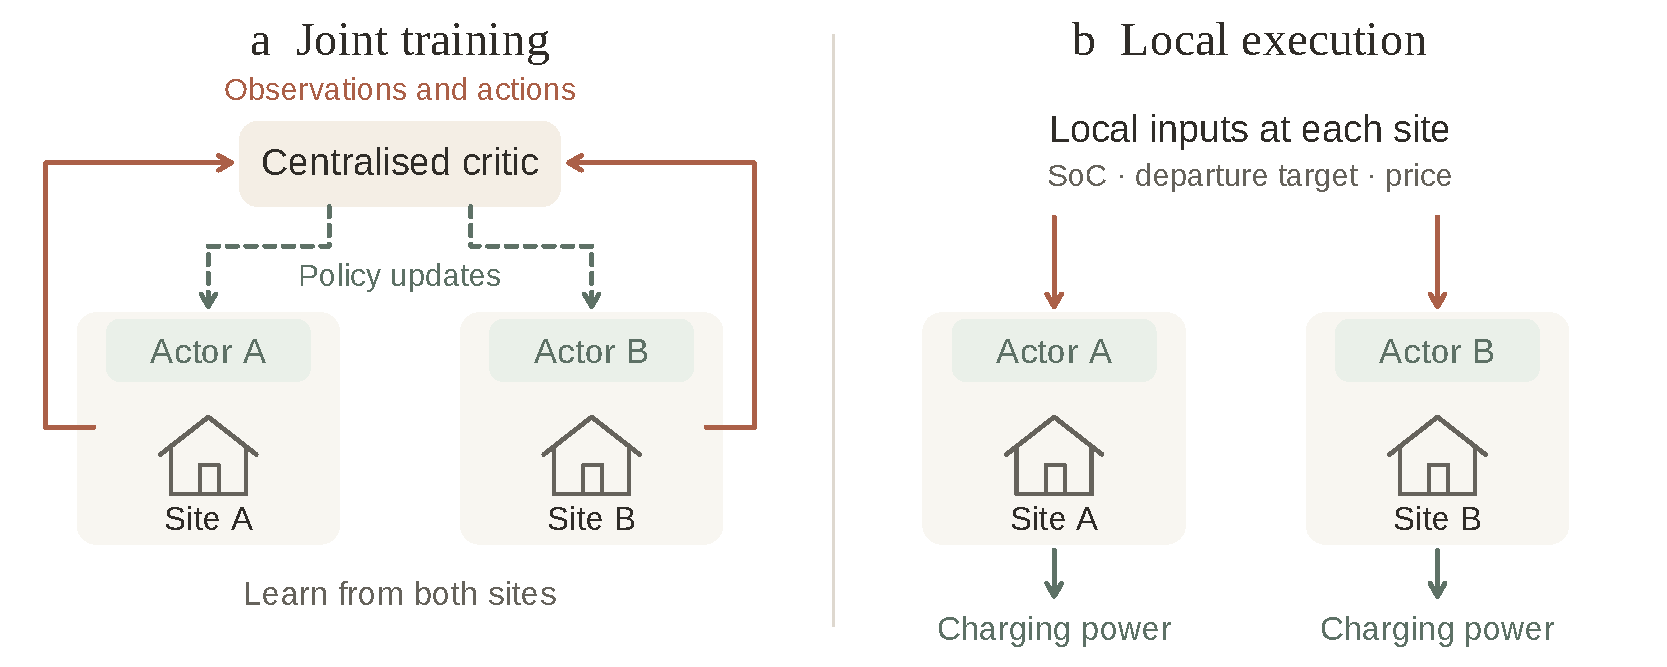
\includegraphics[width=\textwidth]{figures/foundations-ctde.pdf}
\caption{Centralised training and decentralised execution for two sites. Joint observations and actions support policy updates during training; local inputs determine charging decisions during execution. Original illustration based on \textcite{lowe2017maddpg}.}
\label{fig:ch2-ctde}
\end{figure}

\emph{Parameter sharing} allows several agents to use the same policy parameters. Two sites can apply the same charging rule to different \glspl{soc}, prices, and departure times, producing different actions from that common model. Their experience can jointly train the shared rule. The policy uses compatible input and action representations, with asset capabilities or roles included when needed \parencite{albrecht2024marl,yu2022mappo}.

Table~\ref{tab:ch2-learning-organisation} separates these three organisational choices. For example, sites can share policy parameters, train with joint information, and still choose their actions locally during operation.

\begin{table}[!tbp]
\centering\small
\caption{Three organisational choices in multi-agent learning and execution.}
\label{tab:ch2-learning-organisation}
\renewcommand{\arraystretch}{1.16}
\begin{tabularx}{\textwidth}{@{}>{\RaggedRight\arraybackslash}p{0.20\textwidth}>{\RaggedRight\arraybackslash}X>{\RaggedRight\arraybackslash}X@{}}
\toprule
\textbf{Dimension} & \textbf{Choices} & \textbf{\gls{rec}-related interpretation}\\\midrule
Learning information & Local information or information from several agents. & Updates use records from one site or combine observations and actions from several sites.\\\addlinespace[5pt]
Action selection & Centralised or decentralised execution. & One process selects all charging powers, or each site's agent selects its own.\\\addlinespace[5pt]
Policy parameters & Separate or shared parameters. & Agents use separate charging policies or apply the same model to their respective inputs.\\\bottomrule
\end{tabularx}
\end{table}

The next subsection examines how these learning and execution arrangements support coordinated charging, and how a shared outcome can provide useful feedback for the individual decisions that produced it.

\Needspace{7\baselineskip}
\subsection{Coordination and Credit Assignment}
\label{sec:ch2-credit}

The sites' separate charging choices combine into a \gls{rec} demand profile. \emph{Coordination} means that these choices account for their effects on the shared outcome. For example, agents can spread charging across the available low-price intervals while meeting departure targets, reducing the peak created when all vehicles charge together.

\emph{Credit assignment} concerns how a collective result informs the learning of individual agents. If the \gls{rec} peak falls, every agent may receive a better shared reward, although their charging decisions contributed differently to that reduction. Learning needs a way to relate the improvement to those individual choices.

\Needspace{9\baselineskip}
\emph{Counterfactual credit} evaluates one agent's alternatives while holding the other agents' actions fixed. A representative counterfactual baseline $b_i(s,a_{-i})$ is:
\begin{equation}
b_i(s,a_{-i})=
\mathbb E_{a_i'\sim\pi_i}
\left[Q(s,(a_i',a_{-i}))\right],
\label{eq:ch2-counterfactual-baseline}
\end{equation}
Here $a_{-i}$ contains all actions except agent $i$'s, and $Q$ evaluates a joint action in state $s$. The expectation averages over alternative actions $a_i'$ drawn from $\pi_i$, retaining the other agents' actions and the same local information. The difference between the selected joint action's value and this baseline gives agent $i$ an advantage signal \parencite{foerster2018coma}.

\emph{Value decomposition} relates individual utility estimates to a joint action value. Each utility provides a local score for an agent's action, and their combination estimates the collective return. When the combination is monotonic, increasing an individual utility cannot decrease the joint estimate. This property allows each agent to select its highest-scoring action consistently with maximising that estimate \parencite{rashid2018qmix}. In the \gls{rec} example, each site can select a charging action from its local scores while joint training relates their combination to the \gls{rec} outcome.

The next section turns from how agents learn together to the experience available for learning, explaining how policies can be trained from a fixed archive of recorded interactions through offline \gls{rl}.

\FloatBarrier
\section{Offline Reinforcement Learning}
\label{sec:ch2-offline}

The preceding sections described learning through interaction with an environment. \emph{Offline \gls{rl}} instead learns from a fixed dataset of interactions recorded before training begins \parencite{levine2020offline}. The thesis uses this setting to study learning from existing controller records; Section~\ref{sec:ch2-experience-literature} reviews the corresponding methods.

This dataset is an archive of past experience. Each recorded \emph{transition} links an observation or state to the action taken, its reward, and the next observation or state. For a charger, a record might associate the vehicle's \gls{soc} and departure time with the selected power, the charging cost, and the resulting \gls{soc}. Consecutive records can form a trajectory.

The learner repeatedly uses these records to estimate values or improve a policy, without collecting new interactions during training. Figure~\ref{fig:ch2-offline} separates data collection, learning from the fixed dataset, and subsequent use of the policy.

\begin{figure}[!htbp]
\centering
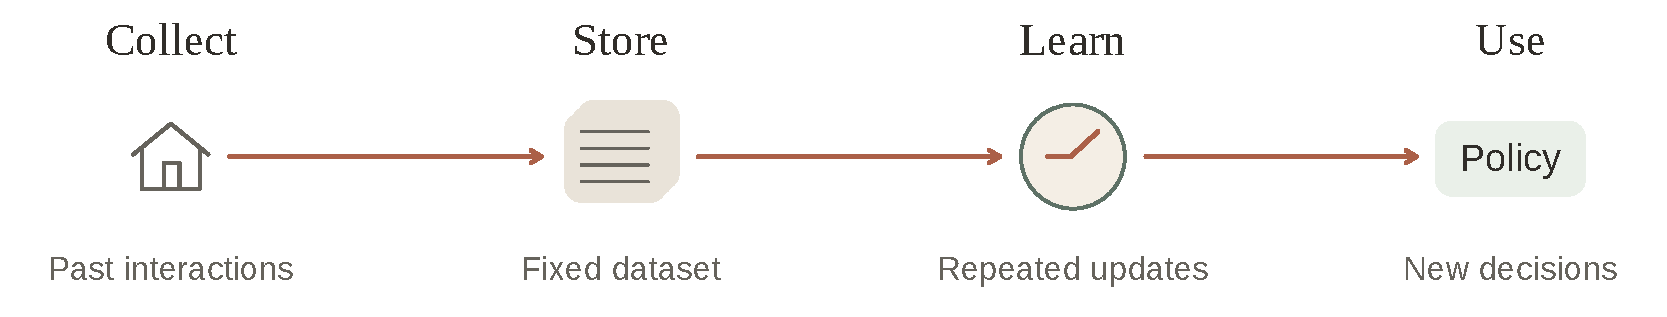
\includegraphics[width=\textwidth]{figures/foundations-offline.pdf}
\caption{Offline learning uses a fixed dataset collected beforehand. The trained policy subsequently receives new observations and selects actions.}
\label{fig:ch2-offline}
\end{figure}

\emph{Off-policy learning}, introduced in Section~\ref{sec:ch2-experience}, separates the policy being improved from the policy that generated the experience. A site can therefore learn from earlier charging decisions made by another controller while continuing to collect new interactions. Offline \gls{rl} uses this separation within a fixed dataset: the learner revisits the same records throughout training, and its updated policy is not used to obtain additional experience during that phase \parencite{levine2020offline}.

The usefulness of the archive depends on its coverage of conditions and decisions. Suppose that the recorded charging controller always starts at maximum power when an \gls{ev} arrives with a low \gls{soc}. Those records provide evidence about immediate charging in that condition, but little direct evidence about postponing it or selecting a lower power. Even a large archive can therefore leave some state--action combinations poorly represented. A new policy may select such combinations, and an inaccurate value estimate can make them appear more attractive than the recorded alternatives. Because offline training collects no additional interactions, the learner cannot test those choices and correct the estimate through new experience. This dependence on dataset coverage motivates the methods reviewed in Section~\ref{sec:ch3-data-prior-knowledge} \parencite{levine2020offline}.

\emph{\gls{bc}} treats each recorded action as a training target. Given the vehicle's condition, the model learns to reproduce the power selected by the collecting controller. Offline \gls{rl} instead uses the recorded rewards and transitions to learn about accumulated performance and improve the policy towards a return objective. Both approaches use past decisions, but their learning signals differ: cloning follows the demonstrated action, whereas offline \gls{rl} evaluates decisions through their recorded consequences.

This section established how recorded experience supports policy learning. The next section turns to how decisions are organised, introducing a hierarchy between \gls{rec} coordination and local control.

\Needspace{8\baselineskip}
\FloatBarrier
\section{Hierarchical Reinforcement Learning and Coordination}
\label{sec:ch2-hierarchy}

\gls{rec} coordination and local control concern different parts of the same charging process. A coordinator may guide when sites consume energy, while each site's controller selects the power requested from its chargers. A \emph{hierarchy} links these responsibilities by making local decisions depend on a higher-level choice. \gls{hrl} learns policies within this organisation. The following subsections explain the levels, timing, and signals used in the thesis, providing the foundations for understanding the methods reviewed in Section~\ref{sec:ch3-hierarchical-controllers}.

\Needspace{7\baselineskip}
\subsection{Decision Levels and Temporal Abstraction}
\label{sec:ch2-temporal-abstraction}

Section~\ref{sec:ch2-community-structure} organised the energy system into assets, sites, and \glspl{rec}, each with its own scope of operation. A control hierarchy assigns decisions across such scopes. In the running example, the \gls{rec} level supplies a coordination signal, and the site level uses that signal alongside its vehicles' requirements to choose charging powers. These responsibilities define the decision levels considered here.

The timing of a decision follows its role in this organisation. A coordinator might update its signal hourly while sites choose charging power every fifteen minutes, making four local decisions under the same signal. The levels can also share a decision interval while retaining different responsibilities.

\emph{Temporal abstraction} groups several elementary steps into one extended behaviour. In the \emph{options} framework, an option has an initiation set describing when it can begin, an internal policy selecting its actions, and a termination rule \parencite{sutton1999options}. A charging option might start when a vehicle connects and end when an energy target is reached or the vehicle departs.

\Needspace{7\baselineskip}
For an option lasting $\tau$ steps, the discounted accumulated reward $R_t^{(\tau)}$ is:
\begin{equation}
R_t^{(\tau)}=\sum_{k=0}^{\tau-1}\gamma^k r_{t+k}.
\label{eq:ch2-option-reward}
\end{equation}
Here $t$ is the starting step, $k$ counts steps within the option, $r_{t+k}$ is the reward following that step's action, and $\gamma$ discounts later rewards. Subsequent value is discounted by $\gamma^\tau$. Variable option durations give the higher-level process a semi-Markov formulation \parencite{sutton1999options}.

These levels and intervals specify when decisions occur. The next subsection explains what the higher-level choice communicates to a local policy.

\Needspace{7\baselineskip}
\subsection{Goals, Skills, and Coordination Signals}
\label{sec:ch2-hierarchy-signals}

A \emph{goal} describes the condition that a local controller should reach. For example, the higher level may assign an amount of energy to deliver before departure. The local policy then determines how charging power develops over the available intervals to pursue that target.

\Needspace{5\baselineskip}
A \emph{skill} provides a policy for a particular behaviour, such as charging steadily or adjusting charging to local generation. Selecting a skill delegates the subsequent power choices to that policy, which responds to the observations it receives. The higher level therefore selects a behaviour whose individual actions are determined locally \parencite{vezhnevets2017fun,nachum2018hiro}.

A \emph{power budget} specifies how much capacity a site can use for a given purpose during an interval. If two chargers share a 6~kW charging budget, the site controller can distribute that power between them according to their remaining energy needs and departure times. The budget sets the combined allowance while leaving the individual allocations to local control.

An \emph{incentive signal}, such as a price multiplier, influences how the local controller assesses possible schedules. A signal that makes the current interval less costly can favour charging during that interval. The resulting power request still follows from the site's conditions, including whether a vehicle is connected and how much energy it requires.

\Needspace{8\baselineskip}
A coordinator policy $\pi_{\mathrm H}$ can select a signal $g_k$ at time $t_k$, which then conditions the local policy $\pi_i$:
\begin{equation}
g_k\sim\pi_{\mathrm H}(\,\cdot\mid o^{\mathrm H}_{t_k}),
\qquad
a_{i,t}\sim\pi_i(\,\cdot\mid h_{i,t},g_k),
\quad t_k\leq t<t_{k+1}.
\label{eq:ch2-hierarchy-policies}
\end{equation}
Here $o^{\mathrm H}_{t_k}$ is the coordinator's observation, $h_{i,t}$ is agent $i$'s local information history, and $a_{i,t}$ is its action. The symbol $\sim$ denotes sampling, and the dot stands for the possible signal or action. The signal remains in use until the next coordinator decision at $t_{k+1}$.

The same incentive can produce different actions. A site with an unmet charging requirement may request power, while another with a fully charged vehicle selects zero. Figure~\ref{fig:ch2-hierarchy} connects these local responses to the shared signal and its update interval.

\begin{figure}[!htbp]
\centering
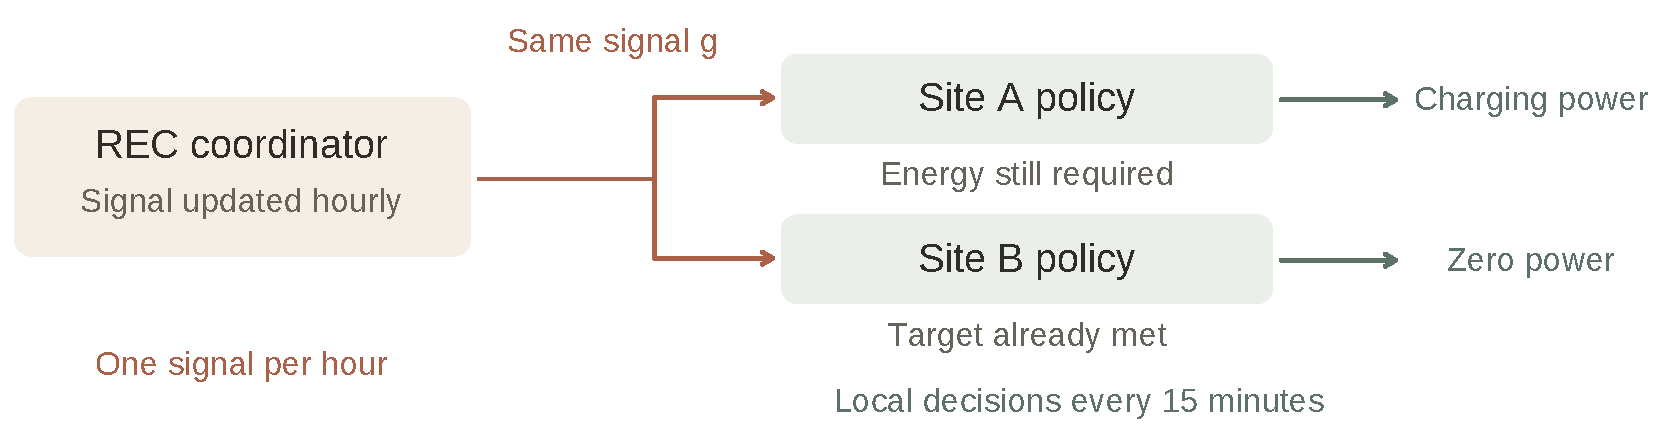
\includegraphics[width=\textwidth]{figures/foundations-hierarchy.pdf}
\caption{One \gls{rec} signal guides successive local decisions. Each site combines it with its own charging conditions to select a power request.}
\label{fig:ch2-hierarchy}
\end{figure}

Hierarchy establishes how decisions are distributed across levels. The next section examines the computation within each policy, from resource observations to the actions returned to individual assets.

\Needspace{8\baselineskip}
\FloatBarrier
\section{Structured Policy Architectures}
\label{sec:ch2-structured}

Section~\ref{sec:ch2-neural} introduced networks that transform numerical inputs into learned representations and outputs. Energy control also gives those quantities a physical organisation, with observations and actions belonging to particular sites and assets. This section develops the entity representations, attention mechanisms, and modular outputs needed to understand the architectures reviewed in Chapter~\ref{chap:related-work} and the method formulations developed in Chapters~\ref{chap:control-benchmark} and~\ref{chap:ti-marl}.

\Needspace{7\baselineskip}
\subsection{Entity and Relational Representations}
\label{sec:ch2-entities}

The numerical inputs introduced in Section~\ref{sec:ch2-neural} must describe the resources whose operation is being controlled. When a site contains several assets, their observations need an arrangement that preserves what each value refers to. A fixed observation vector provides one such arrangement by assigning a declared position to each feature.

For a site with a battery and two chargers, one group of positions can describe the battery and two further groups the vehicles connected to the chargers. The network receives the values in that order. Updating a vehicle's \gls{soc} changes a value; adding a third charger's observations changes the vector's length. The following representations organise these inputs around the resources themselves.

An \emph{entity representation} groups attributes around the resource they describe. Let $x_j$ contain the attributes of entity $j$. An encoder can map each $x_j$ into an embedding, using the same parameters for entities with a common attribute format. Two chargers can therefore use the same encoder while producing different embeddings from their respective \glspl{soc} and departure requirements. The number of entities and the number of attributes describing each entity are separate dimensions.

\Needspace{8\baselineskip}
A \emph{set representation} treats the entities as an unordered collection. One construction uses a shared encoder $\phi$ and an aggregation to produce a site representation $z$:
\begin{equation}
z=\rho\!\left(\sum_{j=1}^{m}\phi(x_j)\right),
\label{eq:ch2-set-representation}
\end{equation}
where $m$ is the number of entities, $\phi(x_j)$ is the embedding of entity $j$, and $\rho$ transforms the sum into the site representation \parencite{zaheer2017deepsets}. Each embedding has a common width, so the sum retains that width as $m$ changes. Adding a compatible charger introduces another application of the encoder and another term in the sum, using the same learned functions.

Reordering the elements leaves this sum unchanged. This property is \emph{permutation invariance}. A site-level value estimate, for example, can describe the same collection whether charger C1 is listed before or after charger C2. The ordering of the records does not change which physical resources are represented.

Resource-specific outputs use the complementary property of \emph{permutation equivariance}. When the input entities are reordered, their corresponding outputs follow the same reordering. If the policy returns one power request per charger, the request for C1 remains associated with C1 after the list order changes. A model can preserve each entity's embedding alongside an aggregate site context to retain this association.

A \emph{graph representation} additionally describes relationships between entities. Nodes can represent a battery, chargers, and their connection point; edges can indicate which assets share that connection. \emph{Message passing} updates a node's representation using information from its neighbours through shared transformations \parencite{gilmer2017mpnn}. In the site example, the connection node can collect information about the assets that draw on its capacity. Figure~\ref{fig:ch2-representations} shows the same resources as a vector, a set, and a graph.

\begin{figure}[!htbp]
\centering
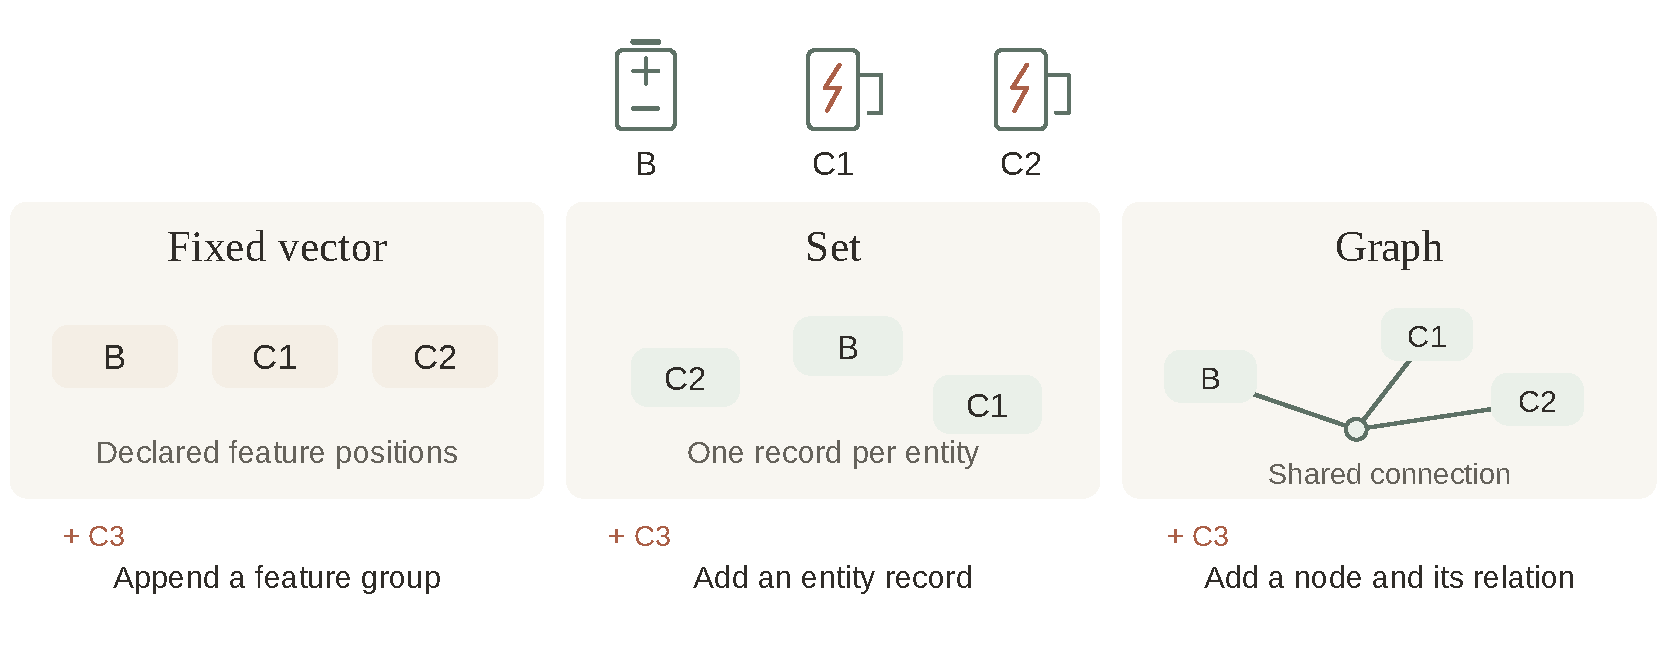
\includegraphics[width=\textwidth]{figures/foundations-representations.pdf}
\caption{Three representations of the same site resources. Vector positions identify feature groups, a set groups attributes by entity, and a graph includes declared relationships. The lower row illustrates adding another charger record.}
\label{fig:ch2-representations}
\end{figure}

\emph{Padding} fills unused positions when several collections are stored in an array with a common allocated size. A presence mask identifies which positions contain entities and which are padding. For example, a batch can allocate four charger positions per site while a mask marks the two populated positions at a particular site. The allocated length, the active entity count, and the embedding width describe different aspects of that representation.

These representations establish which elements enter the policy and how they are associated with resources. The next subsection introduces attention, explaining how the representation of one element can incorporate information from others before decisions are produced.

\Needspace{7\baselineskip}
\subsection{Attention and Transformer Architectures}
\label{sec:ch2-attention}

An entity's decision can depend on information elsewhere in the site. A charger's remaining energy requirement, for example, can be considered alongside another charger's deadline and the available connection capacity. \emph{Attention} forms a weighted combination of input representations, with the weights computed from learned comparisons between them \parencite{vaswani2017attention}.

The computation uses three projections of the available embeddings. A \emph{query} participates in the comparison for the element being updated, while each \emph{key} participates in the comparison for an element whose information may be used. The associated \emph{value} contains the information to combine. For a charger query, matching it against keys from the site produces weights for the corresponding value vectors.

\Needspace{8\baselineskip}
Scaled dot-product attention operates on query, key, and value matrices $Q$, $K$, and $V$:
\begin{equation}
\operatorname{Attention}(Q,K,V)
=\operatorname{softmax}\!\left(\frac{QK^{\mathsf T}}{\sqrt{d_k}}+M\right)V,
\label{eq:ch2-attention}
\end{equation}
where rows of $Q$ contain query vectors, rows of $K$ contain key vectors, and rows of $V$ contain their associated value vectors. The query and key width is $d_k$, and $\mathsf T$ denotes transposition. The optional additive mask $M$ is zero for permitted entries and negative infinity for excluded entries.

The query and key dot products form comparison scores, scaled by $\sqrt{d_k}$. The row-wise softmax turns each query's scores into non-negative weights summing to one over the permitted keys. Multiplication by $V$ then produces one weighted value combination for each query \parencite{vaswani2017attention}.

In \emph{self-attention}, the queries, keys, and values are projected from the same collection. Each site entity can thus receive information from other entities. In \emph{cross-attention}, the queries come from one collection and the keys and values from another. For example, queries associated with requested charging outputs can retrieve information from a collection of observation embeddings.

The number of rows and the width of each row play different roles. In self-attention over $m$ entities, the query and key matrices each have $m$ rows, while their projection widths are architectural choices. Changing $m$ changes the number of comparisons and output representations. A later aggregation can produce a single site representation, or subsequent computation can retain one representation per entity \parencite{lee2019settransformer}.

\emph{Multi-head attention} performs several attention computations using separate learned projections. Their results are concatenated and projected into the output representation. Each head supplies its own combination of values. In the running example, the combined representation draws on several learned comparisons among the same site entities.

A \emph{Transformer block} integrates attention with a feed-forward transformation applied to each element. The feed-forward part transforms the features within an element's representation after attention has combined information across elements. Stacking blocks repeats these operations, producing successive representations of the collection \parencite{vaswani2017attention}.

\emph{Residual connections} add a sublayer's input to its transformed output, retaining a direct path for the incoming representation. \emph{Layer normalisation} normalises features within each element and applies learned scale and offset parameters. Figure~\ref{fig:ch2-attention} relates an attention head to a Transformer block using residual addition and normalisation after each sublayer.

\begin{figure}[!htbp]
\centering
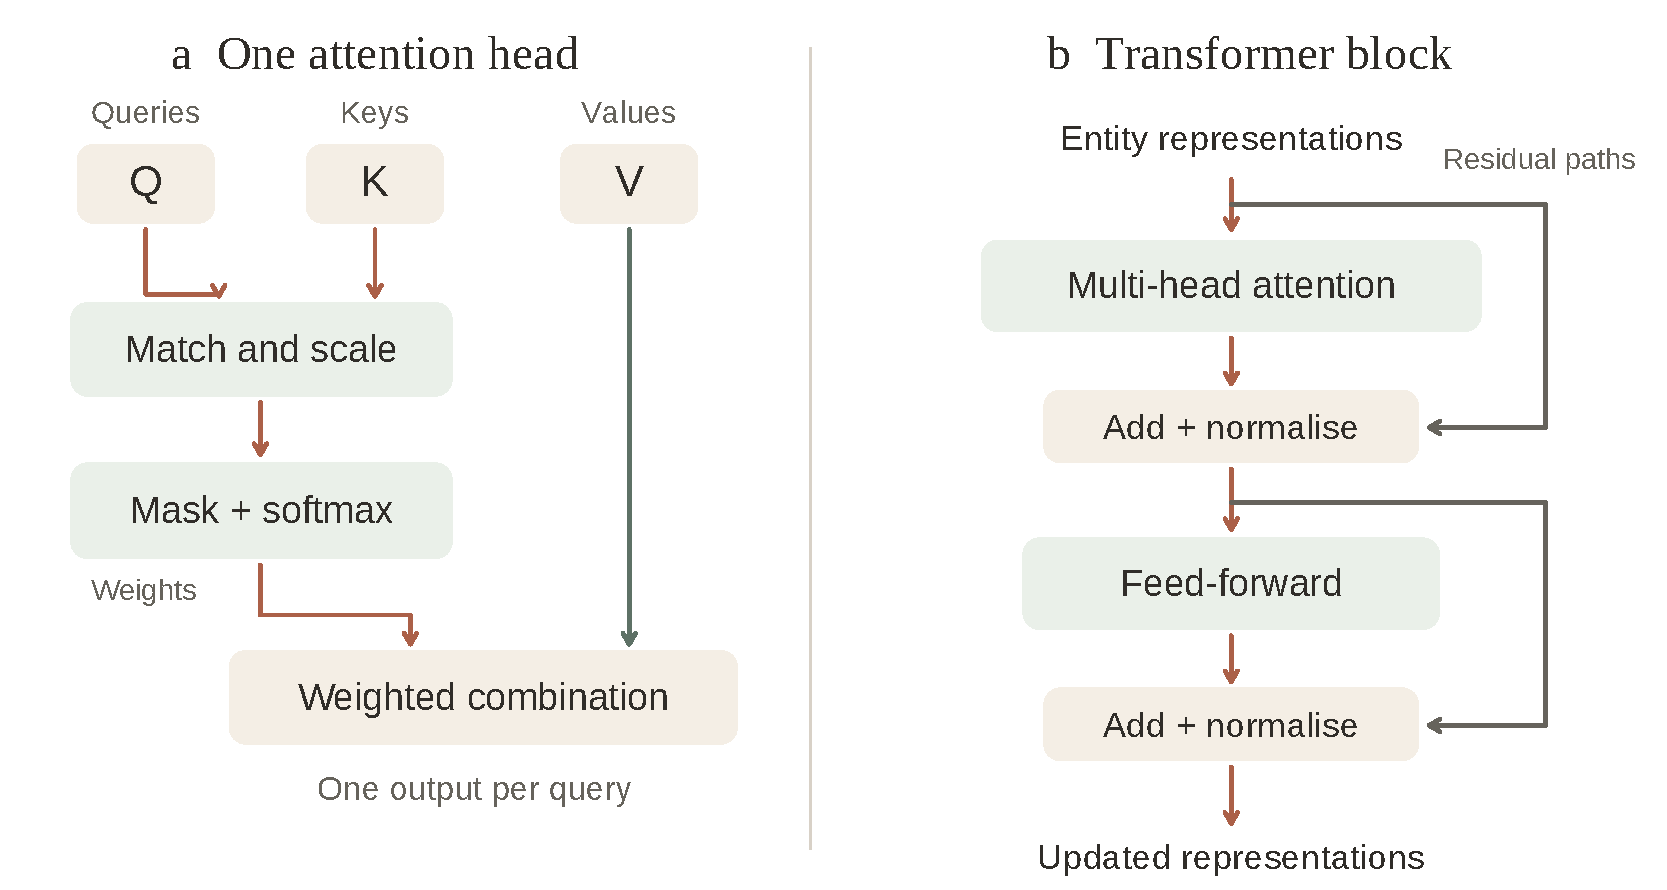
\includegraphics[width=\textwidth]{figures/foundations-attention.pdf}
\caption{Attention and a Transformer block. An attention head computes weights and combines values. Multiple heads form the attention sublayer of the illustrated block; residual paths feed the additions before layer normalisation. Original illustration based on \textcite{vaswani2017attention}.}
\label{fig:ch2-attention}
\end{figure}

Attention and Transformer blocks produce representations that combine the selected information. The next subsection explains how a policy organises those computations into modules and maps their outputs to actions with defined meanings for individual resources.

\Needspace{7\baselineskip}
\subsection{Modular Policies and Action Decoding}
\label{sec:ch2-modular-policies}

A \emph{modular policy} divides its computation into components with specified input or output roles. An encoder can prepare observations, a shared component can combine their representations, and a decoder can produce the quantities used to select an action. Components may be specialised for different resource types or reused across several instances of the same type \parencite{huang2020smp,luketina2025compositional}.

An \emph{output head} maps a representation into a particular group of outputs. A fixed head for two chargers can produce a two-component vector with one power request in each declared position. The number and meaning of those positions belong to the head's specification. This is the output-side counterpart of the fixed feature vector introduced in Section~\ref{sec:ch2-neural}.

A shared resource decoder applies the same function to each resource representation. For three compatible chargers, it produces three outputs, each associated with its source charger. Each evaluation has a fixed output width, while the number of evaluations follows the charger count. Figure~\ref{fig:ch2-modular} illustrates this reuse alongside a separate decoder for another action type.

\begin{figure}[!htbp]
\centering
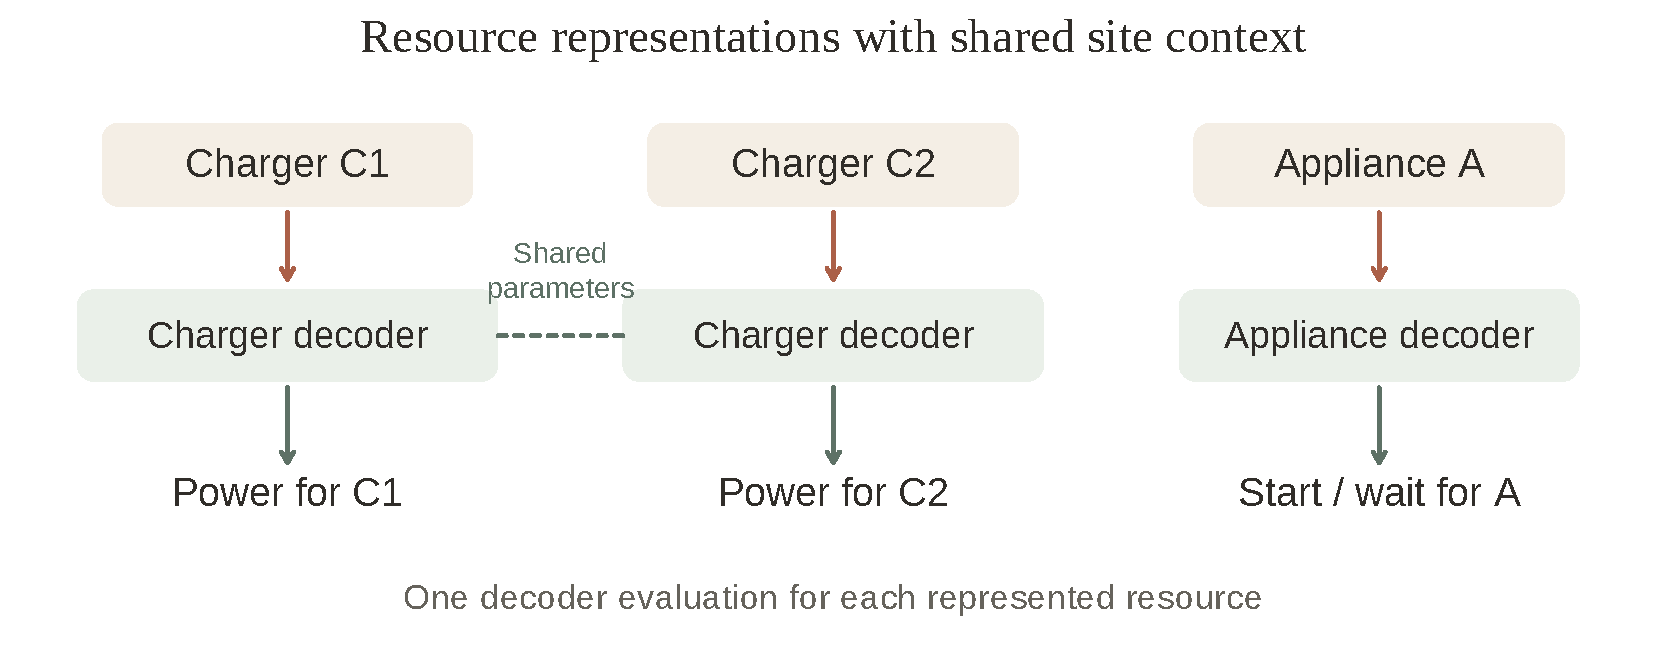
\includegraphics[width=\textwidth]{figures/foundations-modular.pdf}
\caption{Shared decoding with resource-specific outputs. The same charger decoder processes the representations of C1 and C2, producing a separate power request for each. A different decoder produces the appliance's discrete choice. Repeated decoder symbols denote shared parameters.}
\label{fig:ch2-modular}
\end{figure}

A \emph{parameterised action} combines a discrete choice with numerical parameters \parencite{li2022hyar}. A charger might select idle, charge, or discharge, with a power magnitude attached to an active mode. The decoder associates the mode and magnitude with the charger, while conversion to a physical request establishes its units and permitted range.

Resource count and resource type also describe different changes. Adding another charger with the same observation and action format adds another instance of the existing computation. Introducing an asset with a different sensor description or command family changes the input or output mapping required by that type. Type-specific encoders and decoders declare those mappings, while the resource association identifies which instance supplies or receives each quantity.

Structural compatibility concerns whether the architecture can process observations and produce actions for a changed configuration. Control generalisation concerns decision quality and any further learning needed, while computational scalability concerns time and memory requirements as resources increase. A shared decoder can serve a third compatible charger, but its vehicle adds a service request competing for connection capacity. The resulting schedule and additional processing must therefore be assessed. Section~\ref{sec:ch3-scalability} examines these distinctions through the capabilities and evaluation conditions reported in the literature.

The representations, information exchange, and output mappings described here complete the architectural foundations used in the thesis. The chapter summary brings them together with the energy and learning concepts before the next chapter examines the methods built from them.

\FloatBarrier
\section{Chapter Summary}
\label{sec:ch2-summary}

This chapter presented the energy and learning concepts needed to follow the controller formulations developed in the thesis. It began by distinguishing the members of a \gls{rec}, the sites where energy is used, and the assets whose operation can be controlled. Flexibility described the adjustments available within physical limits and service requirements. The charging example illustrated how those adjustments depended on the vehicle's energy needs, connection period, and operating conditions.

Neural networks provided the computational basis for mapping observations to predictions or decisions. The chapter explained how numerical inputs pass through learned intermediate representations to produce outputs, distinguishing changes in input values from changes in the number of components expected by a dense network. These distinctions prepared the later discussion of resource representations.

\gls{rl} placed those decisions within a sequence of actions and consequences. Rewards expressed the objective, returns combined rewards over time, and value functions assessed the expected consequences of following a policy. \gls{marl} extended this account to several interacting agents. In the \gls{rec} example, individually selected charging powers combined into a shared demand profile, connecting local decisions with the need for coordination.

Offline \gls{rl} explained how a policy could be learned from a fixed collection of recorded interactions. Hierarchical control then organised decisions across responsibilities and time scales, with a \gls{rec}-level choice guiding local controllers. The same signal could produce different charging powers because each site also acted on its own vehicle requirements.

Structured policy architectures connected these decision mechanisms to the resources being represented and controlled. Entity-based inputs preserved the association between observations and assets, attention combined information across resources, and shared decoders produced actions for individual instances. The chapter distinguished adding another compatible resource from introducing a new resource type, establishing the concepts needed to discuss changes in a policy's inputs and outputs.

The chapter did not examine the detailed foundations of data acquisition and preparation, state estimation, flexibility prediction, or demand and generation forecasting, because its scope was the learning and decision mechanisms used for \gls{rec} energy control. These subjects remain necessary for other parts of the project, including supplying controller inputs and constructing the experimental setting. Keeping their detailed treatment separate allowed the chapter to follow a continuous path from the energy problem to the formulation of learned decisions.

Chapter~\ref{chap:related-work} now examines how existing methods use these foundations to control energy resources and identifies the gaps that underpin the research problems introduced in Chapter~\ref{chap:introduction}.

\clearpage
\endgroup
